% !TXS template
\documentclass[italian]{article}
\usepackage[T1]{fontenc}
\usepackage[utf8]{inputenc}
\usepackage{lmodern}
\usepackage[a4paper,top=2cm,bottom=2cm,left=1cm,right=1cm]{geometry}
\usepackage[italian]{babel}
\usepackage{enumitem}
\usepackage[fleqn]{amsmath}
\usepackage{amssymb}
\usepackage{mathtools}% http://ctan.org/pkg/mathtools
\usepackage{cancel}
\usepackage{color}
\usepackage[usenames,dvipsnames]{xcolor}
\usepackage{units}
\usepackage{hyperref}
\usepackage{textcomp}
\usepackage{soul}
\usepackage{tikz}
\usetikzlibrary{matrix,decorations.pathreplacing}
\usetikzlibrary{calc}
\usepackage{pifont} %https://www.rpi.edu/dept/arc/training/latex/LaTeX_symbols.pdf

\hypersetup{
	colorlinks,
	citecolor=black,
	filecolor=black,
	linkcolor=black,
	urlcolor=black
}

\author{Giacomo De Liberali}

\renewcommand{\labelitemii}{$\circ$}
\newcommand{\tab}{\qquad\quad}
\newcommand{\mmod}{\text{ mod }}
\newcommand{\mcd}[2]{\text{$\text{MCD}(#1, #2)$}}
\newcommand{\mcm}[2]{\text{$\text{mcm}(#1, #2)$}}
\newcommand{\N}{\text{$\mathbb{N}$}}
\newcommand{\divides}[2]{\text{$#1 \;|\; #2$}}
\newcommand{\notdivides}[2]{\text{$#1 \not|\; #2$}}

\newcommand{\linea}{\begin{center}\rule{5cm}{1pt}\end{center}}


\newcommand{\congruente}[1]{\text{$\equiv_{#1}\;$}}

\newcommand{\crossmark}{\textcolor{red}{\text{$\qquad$\ding{56}}}}
\renewcommand{\checkmark}{\textcolor{ForestGreen}{\text{$\qquad$\ding{52}}}}

\newcommand{\tright}[1]{\hfill #1 \\}
\newcommand{\rtext}[1]{\hfill #1 \\}

\newcommand{\ins}[1]{\text{$\mathbb{#1}$}}

\newcommand{\combs}[2]{\text{$C_{#1,#2}$}}
\newcommand{\combr}[2]{\text{$C'_{#1,#2}$}}
\newcommand{\disps}[2]{\text{$D_{#1,#2}$}}
\newcommand{\dispr}[2]{\text{$D'_{#1,#2}$}}

\begin{document}
	
\title{Matematica discreta}
\maketitle

\tableofcontents
\pagebreak
\section{Insiemistica}
\subsection{Operazioni}
\begin{itemize}
	\item Unione - $A\cup B=\{x:x\in A\lor x\in B\}$
	\item Intersezione - $A\cap B=\{x:x\in A\land x\in B\}$
	\item Complementazione - $A\backslash B=\{x:x\in A\land x\notin B\}$
	\item Prodotto cartesiano - $A\times B=\{(x,y):x\in A,y\in B\}$
\end{itemize}

\textit{Tutte queste regole seguono le logiche dell'algebra booleana (Boole).}\\

\subsection{Leggi di De Morgan}
\begin{itemize}
	\item Idempotenza:
	
	\begin{itemize}
		\item $A\cup A=A$
		\item $A\cap A=A$
	\end{itemize}
	\item Associatività:
	
	\begin{itemize}
		\item $A\cup(B\cup C)=(A\cup B)\cup C$
		\item $A\cap(B\cap C)=(A\cap B)\cap C$
	\end{itemize}
	\item Commutabilità:
	
	\begin{itemize}
		\item $A\cup B=B\cup A$
		\item $A\cap B=B\cap A$
	\end{itemize}
	\item Distributività:
	
	\begin{itemize}
		\item $A\cup(B\cap C)=(A\cup B)\cap(A\cup C)$
		\item $A\cap(B\cup C)=(A\cap B)\cup(A\cap C)$
	\end{itemize}
	\item Assorbimento:
	
	\begin{itemize}
		\item $A\cup(A\cap B)=A$
		\item $A\cap(A\cup B)=A$
	\end{itemize}
	\item Complementazione:
	
	\begin{itemize}
		\item $(X\backslash A)\cup A=X$ con $A\subseteq X$
		\item $(X\backslash A)\cap A$= $\textrm{Ø}$
	\end{itemize}
\end{itemize}
\begin{itemize}
	\item Altre leggi
	\begin{itemize}
			\item $(A\cup B)'=A'\cap B'$
			\item $(A\cap B)'=A'\cup B'$
	\end{itemize}
\end{itemize}

\pagebreak
\subsection{Operatori matematici}
\begin{itemize}
	\item AND: $\land$
	\item OR: $\lor$
\end{itemize}

\subsection{Teorema}
$A\cup(A\cap B)=A$

\emph{Prova: siano A e B insiemi} \textit{[una dimostrazione si inizia sempre così]}

$C\subseteq D\land D\subseteq C\Rightarrow C=D$
\begin{itemize}
	\item (I) $A\subseteq A\cup(A\cap B)$
	\begin{itemize}
		\item $x\in A \Rightarrow x \in A \cup (A\cap B)$ [\textbf{vero} per definizione di unione]
	\end{itemize}
	\item (II) $A\cup (B\cap C) \subseteq A$
	\begin{itemize}
		\item $x \in A\cup (B\cap C) \Rightarrow x \in A$
		\begin{enumerate}[label=(\alph*)]
			\item $x\in A \Rightarrow x \in A$ [\textbf{vero}]
			\item $x\in A \cup B \Rightarrow x \in A \land x\in B \Rightarrow x\in A$ [\textbf{vero}]
		\end{enumerate}
	\end{itemize}
\end{itemize}

\subsection{Teorema}
$A\cap (B\cup C)=(A\cap B)\cup (A\cap C)$ \emph{[verifico che sia vero]}

Prova: siano A,B e C insiemi\textit{[prendo un elemento arbitrario dal primo insieme e verifico sia presente anche negli altri]}

\begin{itemize}
	\item (I) $A\cap (B\cup C)=(A\cap B)\cup (A\cap C)$
	\begin{itemize}
		\item $x \in A \cap (B\cup C) \Rightarrow x\in A \land x\in B\cup C$
		\item $x\in B\cup C \Rightarrow x\in B \lor x\in C$
		\item Posso suppore che:
		\begin{enumerate}[label=(\alph*)]
			\item $x\in B \Rightarrow x\in A\cap B \Rightarrow x\in (A\cap B) \cup (A\cap C)$ [poiché è un sottoinsieme]
			\item $x\in A\cap C \Rightarrow x\in (A\cap C)\cup (A\cap B)$ [poiché è un sottoinsieme]
		\end{enumerate}
	\end{itemize}
	\item (II) $(A\cap B)\cup (A\cap C) \subseteq A \cap (B\cup C)$
	\begin{enumerate}[label=(\alph*)]
		\item $x\in A\cap B \Rightarrow x\in A \land x\in B$
		\begin{itemize}
			\item $x\in B \Rightarrow x\in B\cup C \Rightarrow x\in A\cap (B\cup C)$
		\end{itemize}
		\item $x\in A\cap C \Rightarrow x\in A \land x\in C$
		\begin{itemize}
			\item $x\in C \Rightarrow x\in (B\cup C) \Rightarrow x\in A\cap (B\cup C)$ [fine dimostrazione]
		\end{itemize}
	\end{enumerate}
\end{itemize}
\pagebreak
\section{Relazioni}

Una relazione non è una funzione quando dato un input ricevo più output.\\

\_essere studenti di professore\_ \emph{[relazione binaria, non è una funzione]}

Dominio = studenti, Codominio = professori

(Marco, Simeoni)$\in$Relazione? Si. \\

Una relazione binaria R di dominio A e codominio B è un sottoinsieme di $A\times B$:
\begin{center}
	$Relazione\subseteq Studenti \times Professori$
\end{center}

$\{(x,y)\in Relazione : x \in Studenti \land y \in Professori \land \textit{x è uno studente del professore y}\}$ \\ 
\pagebreak
\section{Funzioni}
Una relazione è una funzione quando ad ogni elemento del dominio corrisponde un solo elemento del codominio.\\ \\
Una funzione
\[f: A\rightarrow B\]
è una relazione binaria
\[(f\subseteq A\times B)\]
tali che per ogni $a\in A$ esiste un \underline{unico} elemento $b\in B$ tali che $(a,b)\in R$.\\\\
\textbf{06$\cdot$10$\cdot$2015}
\[R=\{(x,y):x,y\in A \land \textit{x ha la stessa altezza di y}\}\]
dove A è l'insieme delle persone presenti in questo momento in aula 1.\\ \\
Una funzione è tale solo se dato un input ricevo un \underline{solo} output.\\
Esempio:
\[
	R=\{(x,y):x\in \mathbb{Z}, y\in \mathbb{N} \land x=y^2\}
\]
Non è una funzione, in quanto $\nexists \; y : (2,y)\in \mathbb{R}$ \emph{[non esiste un numero naturale la cui radice sia 2]} \\
\subsection{Funzioni iniettive e surgettive}
Una funzione $f:A\to B$ è iniettiva se per ogni $x,y \in A$ abbiamo che
\[
	f(x)=f(y)\Rightarrow x=y
\] \\
Una funzione è surgettiva se per ogni $y\in B$ esiste un $x\in A$ tale che
\[
	f(x)=y
\] \\\\
Siano $A$ e $B$ insiemi finiti. Se $f: A\to B$ è:
\begin{itemize}
	\item iniettiva, allora $|A|\leq|B|$ \qquad \emph{dove |A| è la cardinalità di A, numero di elementi}
	\item suriettiva, allora $|B|\leq |A|$
	\item bigettiva, allora $|A|=|B|$
\end{itemize}
Una funzione $f:A\to B$ è invertibile se esiste $g$ tale che $B\to A$: 
\[
	f\circ g \qquad \text{\emph{[f composto g, ovvero applico prima g e poi f]}}
\] \\\\
Una funzione $f:A\to B$ è bigettiva se $f$ è invertibile.\\
$f:A\to B$ è invertibile se esiste $g: B\to A$ tale che
\[
	g\circ f = I_A \qquad \qquad f\circ g = I_B 
\]
\[
	\underbrace{A \xrightarrow[]{f} B \xrightarrow[]{g} A}_{
		\text{identità di A, $I_A$}} \text{\qquad}	
	\underbrace{B\xrightarrow[]{g} A \xrightarrow[]{f} B}_{
		\text{identità di B, $I_B$}}
\]
\pagebreak \\
\textbf{Dimostrazione}\\
Supponendo che $f:A\to B$ sia bigettiva [stessa cardinalità].\\
$g: B\to A$ \qquad $g(y)=x \quad \text{dove } x \text{ è l'elemento di } A \text{ tale che } f(x)=y \text{ dove } y\in B$ 
\begin{gather*}
	(g\circ f)x = g(f(x)) \quad \text{con } x\in A \\
	(f\circ g)x = f(g(x)) \quad \text{con } y\in B
\end{gather*}
Supponiamo $f$ sia invertibile:\\
allora esiste $g: B \to A$ tale che $g\circ f=I_A \qquad f\circ g = I_B$\\
Poniamo che $f$ sia iniettiva:
\begin{gather*}
	f(x) = f(y) \Rightarrow x=y \qquad \text{ con } x,y \in A \\
	g(f(x))=g(f(y)) \to \underbrace{(g\circ f)x}_{I_A(x)=x} = \underbrace{(g\circ f)y}_{I_B(y)=y}
\end{gather*}
Poniamo che $f$ sia surgettiva: per ogni $y\in B$ esiste $x\in A$ tale che $f(x)=y$\\
\begin{center}
	$f(\underbrace{g(y)}_{A})y=y$
\end{center}
\pagebreak
\subsection{Tutorato}
Una funzione $f$ associa ad ogni elemento di un insieme $A$, detto dominio, uno ed un solo elemento dell'insieme $b$, detto codominio:
\[f: A \longmapsto B\]
Esempio pratico:
\begin{gather*}
	A=\{a,b,c,d\}\\
	B=\{1,2,3\}
\end{gather*}
$f(a) = 1$, dove 1 è l'immagine di $a$ e $a$ è la controimmagine di $1$.\\\\
\textbf{Funzioni iniettive}\\
Una funzione $f$ è iniettiva se ogni elemento del codominio è mappato al massimo da un elemento del dominio.\\Se $\underbrace{|B|<|A|}_{cardinalità}$ non può essere iniettiva.\\\\
\textbf{Funzioni suriettive}\\
Una funzione $f$ è surgettiva se ogni elemento del codominio è mappato da almeno un elemento del dominio.\\Se $|B|>|A|$ non può essere surgettiva.\\\\
\textbf{Funioni bigettive}\\
Una funzione $f$ è surgettiva quando è sia iniettiva che surgettiva, ovvero quando ogni elemento del codominio è mappato esattamente da un elemento del dominio. Può essere bigettiva solo se $|A|=|B|$\\\\
\textbf{Esempi}:\\
\begin{gather}
	f: \mathbb{Z}\longmapsto \mathbb{N} \qquad f(x) = abs(x) \qquad [\textit{suriettiva}]\\
	f: \mathbb{N}\longmapsto \mathbb{N} \qquad f(x) = x+1 \qquad [\textit{iniettiva}] \\
	f: \mathbb{Z}\longmapsto \mathbb{Z} \qquad f(x) = x+1 \qquad [\textit{bigettiva}]\\
	f: \mathbb{Z}\longmapsto \mathbb{Z} \qquad f(x) = x^2 \qquad [\textit{ne iniettiva ne suriettiva}] \\
	f: \mathbb{R}\longmapsto \mathbb{R} \qquad f(x) = x^2 \qquad [\textit{ne iniettiva ne suriettiva}] \\
	f: \mathbb{N}\longmapsto \mathbb{N} \qquad f(x) = x^2 \qquad [\textit{iniettiva ma non suriettiva}]
\end{gather}

\pagebreak
\subsection{Ordinamenti parziali}
Proprietà degli ordinamenti parziali sui numeri naturali:
\begin{itemize}
	\item $x\leq y \text{ sse } \exists z (x+z=y)$
	\item proprietà riflessiva: $\forall x (x\leq x)$
	\item proprietà transitiva: $\forall xyz (x\leq y \land y\leq z \Rightarrow x\leq z)$
	\item proprietà antisimmetrica: $\forall xyz (x\leq y \land y\leq x \Rightarrow x=y)$
\end{itemize}
\pagebreak
\section{Principio di induzione}
Serve per verificare che una certa proprietà valga per tutti gli elementi di un insieme. Data una proposizione $P$, se $P$ vale per $x_0$, bisogna dimostrare che P vale anche per $x+1$, ovvero che P valga per tutti gli elementi:
\begin{center}
	$P(x_0) \land \left(P(k)\to P(k+1)\right) \to \forall x \geq x_0, P(x)$
\end{center}
Esempio: 
$\{x:x\in \mathbb{N}, x \text{ è primo}\} \leq \mathbb{N} \to \underline{P}$ \\
\[
\underbrace{\underline{P}(0)}_{\text{[0 ha la proprietà \underline{P}]}} \text{ e } \forall x (\underline{P}(x)\Rightarrow\underline{P}(x+1)) \Rightarrow \forall x \quad \underline{P}(x)
\]
\emph{[se $x$ ha la stessa proprietà \underline{P} e $x+1$ ha la stessa proprietà, essa vale per l'intero campo numerico]}
\subsection{Esercizi}
\subsubsection{Esercizio 1}
Dimostrare che
\[
	\sum_{i=0}^{x}i = 1+2+3+\dots + (x-1) + x = \frac{x(x+1)}{2}
\]
vale per ogni $x\in \mathbb{N}$.\\
Inizio dimostrazione:
\[
	\underline{P}(x) \text{ sse } \sum_{i=0}^{x} i=\frac{x(x+1)}{2}
\]
\[
	\underline{P}(0) = \sum_{i=0}^{0}i=\frac{0(0+1)}{2} = 0 \qquad \text{vero}
\]
Supponiamo per ipotesi di induzione che $x$ abbia la proprietà $\sum_{i=0}^{x} i=\frac{x(x+1)}{2}$\\
\[
	\sum_{i=0}^{x+1}i=\frac{(x+1)(x+2)}{2} \to \sum_{i=0}^{x} i + (x+1) \to \underbrace{\frac{x(x+1)}{2}}_{\text{induzione}} + (x+1) 
\]
\[
	\to \frac{x(x+1)+2(x+1)}{2} \to \frac{(x+1)(x+2)}{2} \qquad \text{ dimostrato.}
\]
\pagebreak
\subsubsection{Esercizio 2}
Dimostrare che
\[
	\sum_{k=0}^{x}(2k+1)=(x+1)^2
\]
Studio risoluzione:\\
$1 \qquad 3 \qquad 5 \qquad 7 \qquad \dots$\\
$7 \qquad 5 \qquad 3 \qquad 1 \qquad \dots$\\
$8 \qquad 8 \qquad 8 \qquad 8 \qquad \dots$
\[
	\sum_{k=0}^{3}(2k+1)=1+3+5+7=16	
\]
Inizio dimostrazione per induzione. Base 0:
\[
	\sum_{k=0}^{0}(2k+1)=(0+1)^2=1 \qquad \text{vero}
\]
La base è valida, supponiamo per induzione che $\sum_{k=0}^{x}(2k+1)=(x+1)^2$
\[
	\sum_{k=0}^{x+1}(2k+1)=\biggl ( \sum_{k=0}^{x}(2k+1) \biggl ) + (2(x+1)+1) = (x+1)^2 + 2(x+1)+1 = \underbrace{((x+1)+1)^2}_{\text{prodotto notevole}} \qquad \text{[dimostrato]}
\]
Se la proprietà vale per $x+1$, vale per l'intero campo numerico!
\pagebreak
\subsubsection{Esercizio 3}
Dato un insieme A di cardinalità $n$, allora $\mathcal{P}(A)=\{B:B\subseteq A\}$ ha cardinalità $2^n$, dove $\mathcal{P}(A)$ è l'insieme delle parti di $A$.\\\\
\textbf{Caso base}: $n=0$
\begin{gather*}
	\text{Se } n=0 \text{, } A=\varnothing \text{. } \text{Se } A=\varnothing \text{, l'insieme delle parti di } A [\mathcal{P}(A)]\text{ vale } \{\varnothing \}.\\
	2^0 = 1 \to 2^0 = 1 \qquad [vero]
\end{gather*}
Dato che il caso base è vero, inizio la dimostrazione:\\
\textit{Supponiamo per ipotesi di induzione che l'insieme delle parti di un insieme di cardinalità n abbia cardinalità $2^n$.}
\begin{gather*}
	|\mathcal{P}(A)|=2^{n+1} \\
	\textit{prendo } B\subseteq A \to  a_{n+1} \in B?\;\\
	\textit{Partiziono $\mathcal{P}(A)$ in sottoinsiemi che contengono } a_{n+1} \textit{ e quelli che non contengono } a_{n+1}	\\
	A = \{a,b,c\} \qquad \to \textit{fisso l'ultimo elemento [$c$]} \\
	\mathcal{P}(A)=\{\varnothing, \{a\}, \{b\}, \{c\}, \{a, c\}, \{b,c\}, \{a,b,c\}\}\\
	\text{Partizioni che contengono l'ultimo elemento: } 
	\{c\}, \{a,c\}, \{b,c\},\{a,b,c\} \to 4 \text{ elementi } \to 2^2\\
	\text{Partizioni che \underline{non} contengono l'ultimo elemento: } 
	\{\varnothing\}, \{a\}, \{b\},\{a,b\} \to 4 \text{ elementi } \to 2^2
\end{gather*}
Esempio riportato al caso generico: $2^n+2^n = 2^{n+1}$
\begin{gather*}
	\{B:B\subseteq A \land a_{n+1} \in B\} \\
	\{B:B\subseteq A \land a_{n+1} \notin B\} \\
\end{gather*}
L'insieme delle parti di $A$ è l'unione dei due insiemi sopracitati.\\\\
Se $f$ è iniettiva suppongo che:
\[
	f(b) = f(c) \xrightarrow{implica} B=C
\]
Sfrutto la definizione di $f(b)$ e ottengo:
\begin{gather*}
	B \diagdown \{a_{n+1}\} = C\{a_{n+1}\} \\
	B \diagdown \{a_{n+1}\} \cup \{a_{n+1}\} = B \to C \diagdown \{a_{n+1}\} \cup \{a_{n+1}\} = C
\end{gather*}
segue che $B=C$ e $f$ è iniettiva:
\[
	f: \{B:B\subseteq A \land a_{n+1} \in B\} \longmapsto \{B\subseteq A : a_{n+1} \notin B\}
\]\\
\pagebreak
\subsubsection{Esercizio 4}
Dimostrare che:
\[
	\text{per ogni } n\geq 1 \text{ si ha } 2^n \geq n+1
\]
\textbf{Caso base}: $n=1$\\
\[
	2^1 = 1 +1 = 2 \xrightarrow{equivale} 2^1=2 \qquad [\textit{vero}]
\]
Dato che la verifica del caso base è andata a buon fine, iniziamo la dimostrazione.\\
\textit{Suppongo per induzione che} $2^n \geq n+1$ sia vero
\begin{gather*}
	2^{n+1}=2\cdot2^n \xrightarrow{\textit{per induzione}} 2\cdot 2^n \geq 2\cdot (n+1) = 2n + 2 = (n+2)+n \to \underbrace{(n+2)+n \geq n+2}_{\text{perché } n \geq 1} \Rightarrow 2\cdot 2^n \geq n+2 \\
\end{gather*}
Fine, dimostrato.

\subsubsection{Esercizio 5}
Dimostrare che:
\[
\text{per ogni } n\geq 0 \text{ si ha che } 8 \text{ divide } (3^{2n}-1)
\]
\textbf{Caso base}: $n=0$\\
\[
3^{2\cdot 0} -1 = 0 \qquad [\textit{vero, ogni numero divide 0}]
\]
Dato che la verifica del caso base è andata a buon fine, iniziamo la dimostrazione.\\
\textit{Suppongo per induzione che} $8 \underbrace{|}_{divide} \textcolor{blue}{(3^{2n} - 1)}$ sia vero. Dimostro che $(3^{2(n+1)} - 1)$ sia divisibile per 8.
\begin{gather*}
	3^{2n+2} - 1 = 3^{2n}\cdot 3^2 - 1 \xrightarrow{\textit{per induzione}} (3^{2n}\underbrace{-1+1}_{\textit{li aggiungo}})\cdot 3^2 - 1 = \\
	= \underbrace{\textcolor{blue}{(3^{2n}-1)}}_{\textit{induzione}}\cdot (3^2)+\underbrace{(3^2-1)}_{8 \; | \; 8 \to \textit{vero}}
\end{gather*}
E' divisibile per 8 in quanto un numero divisibile per 8 (l'induzione) moltiplicata per una costante $k$, resta divisibile per 8. Se a questo valore aggiungiamo un multiplo di 8 (oppure 8 stesso), otteniamo nuovamente un numero $d$ divisibile per 8. Segue
\[
	d=k\cdot n
\]
dove $n$ è multiplo di 8, $k$ è una costante $\in \mathbb{N}$.
\pagebreak
\subsection{Tutorato}
Dimostrare per induzione $\forall x \geq x_0, P(x)$:
\begin{enumerate}
	\item Caso base $P(x_0)$
	\item Assumiamo che la proprietà sia vera per un certo $k$, cioè che $P(k)$ sia vera (ipotesi di induzione)
	\item Per il principio di induzione la proprietà è vera $\forall x \geq x_0$
\end{enumerate}
\subsubsection{Esempio - numeri binari}
\[
	\begin{cases*}
		\overbrace{11}^{2} = 2^0 + 2^1 = 3 = 2^2 -1 \\
		\underbrace{111}_{3} = 2^0 + 2^1 + 2^2 = 7 = 2^3 -1
	\end{cases*}
\]
\begin{gather*}
	P(n): \sum_{i=0}^{n-1}2^i = 2^n - 1 \qquad \forall n \geq 1
\end{gather*}
Caso base: n=1
\[
	P(1)=\sum_{i=0}^{0}2^i=2^0=1 \xrightarrow{equivale} 2^1 -1 = 0 \qquad [vero]
\]
Assumiamo $P(k) \to \sum_{i=0}^{k-1}2^i = 2^k -1$. Dobbiamo dimostrare che $P(k+1) \to \sum_{i=0}^{k+1-1}2^i=2^{k+1}-1$
\begin{gather*}
	\begin{split}
		2^{k+1}-1 & = 2^k\cdot 2 - 1 \\
		& = 2^k + 2^k -1 \\
		& = 2^k + \underbrace{\sum_{i=0}^{k-1}2^i \Rightarrow 2^0 + 2^1 + \dots + 2^{k-1} + 2^k}_{\textit{per ipotesi di induzione}} \\
		& = \sum_{i=0}^{k+1-1}2^i=2^{k+1}-1
	\end{split}
\end{gather*}
Per il principio di induzione $\forall x \geq 1, P(k) $ vale. 

\pagebreak
\subsubsection{Esempio}
Dimostrare che $\forall n \geq 4$
\[
	\left(	\sum_{i=1}^{n}i \right) \leq n(n+1) \leq n!
\]
Base: $n=4$
\[
	\sum_{i=1}^{4} = 1 + 2 + 3 + 4 \leq 4\cdot 5 \leq 4! \to 10\leq20\leq 24 \qquad vero
\]
Inizio la dimostrazione per $n+1$, visto il caso base
\begin{gather*}
	\sum_{i=1}^{n+1}i \leq (n+1)(n+2) \leq (n+1)! \\
	\sum_{i=1}^{n}i + (n+1) \leq n(n+1)+2(n+1) \leq n!\cdot(n+1) \\
	\dots
\end{gather*}

\subsubsection{Esempio}
Dimostrare che $\forall n \geq 1$
\[
	\left(	\sum_{i=1}^{n}(2i - 1)\right) = n^2
\]
Base: $n=1$
\[
	\sum_{i=1}^{1}(2i-1) = 2 - 1 = 1 = 1^2 \qquad vero
\]
Vista la base inizio la dimostrazione
\begin{gather*}
	\sum_{i=1}^{n+1}(2i - 1) = (n+1)^2 \\
	\sum_{i=1}^{n}(2i - 1) + 2(n+1)-1 = (n+1)^2 \\
	\underbrace{n^2}_{\text{induzione}} + 2n + 1 = (n+1)^2 \\
	(n+1)^2 = (n+1)^2
\end{gather*}
\pagebreak
\subsubsection{Esempio}
Dimostrare che $\forall n \geq 3$
\[
	2n+1 \leq2^n
\]
\dots
\subsubsection{Esempio}
Dimostrare che $\forall n \geq 6$
\[
	5n + 5 \leq n^2
\]
Base: $n=6$
\[
	5\cdot 6 + 5 \leq 6^2 \qquad vero
\]
Vista la base inizio la dimostrazione
\begin{gather*}
	5(n+1)+5\leq(n+1)^2 \\
	\text{Semplifico il termine a sinistra: }
	5(n+1) + 5 = \underbrace{5n + 5}_{\text{forma inziale}} + 5
\end{gather*}
Sommando o sottraendo lo stesso termine a destra e a sinistra di una disuguaglianza si ottiene la medesima disuguaglianza
\begin{gather*}
	5n + 5 + 5 \leq n^2 + 5 \\
	5n + 5 + 5 \leq n^2 + 2n + 1 \\
	5 \leq 2n + 1 \qquad \text{vero}
\end{gather*}

\subsubsection{Esempio: n divisibile per x}
Dimostrare che $\forall n \in \mathbb{N}$
\[
	n^3 + 2n \text{ è divisibile per } 3
\]
Base: $n=0$
\[
	0^3 + 2\cdot 0 = 0 \underbrace{\;|\;}_{divide} 3 \qquad \text{vero, ogni numero divide 0}
\]
Vista la base inizio la dimostrazione
\begin{gather*}
	(n+1)^3 + 2(n+1) \\
	n^3 + 3n^2 + 3n + 1 + 2n + 2 \\
	n^3 + 2n + 3n^2 + 3n + 3 \\
	\underbrace{(n^3+2n)}_{\text{per induzione è divisibile per 3}} + \qquad \underbrace{3(n^2 + n + 1)}_{\text{divisibile per 3}} \qquad vero
\end{gather*}
\pagebreak
\subsubsection{Esempio: funzioni ricorsive}
Dimostrare che 
\begin{gather*}
	f(n)
	\begin{cases*}
		3 \qquad \textit{con } n=1 \\
		5 \qquad \textit{con } n=2 \\
		3f(n-1)-2f(n-2)
	\end{cases*}
\end{gather*}
è uguale a 
\[
	g(n) = 2^n + 1
\]
Inizio la dimostrazione verificando il caso base:
\begin{gather*}
	n=1 \qquad 2^1 + 1 = 3 \checkmark \\
	n=2 \qquad 2^2 + 1 = 5 \checkmark
\end{gather*}
I casi base sono veri, quindi suppongo vero
\[
	f(x) = g(x) = 2^n + 1 \qquad \forall i(1\leq i\leq k), k\in \mathbb{N}
\]
Devo dimostrare ora che l'uguaglianza vale anche per $(x+1)$:
\begin{gather*}
	\begin{split}
		f(x+1) = 3f(k)-2f(k-1) &= g(k+1)\\
		&= 3g(k) - 2g(k-1) \qquad \text{per ipotesi di induzione forte} \\
		&= 3(2^k+1)-2(2^{k-1}+1) \\
		&= 3\cdot 2^k + 3 -2\cdot 2^{k-1} - 2 \\
		&= 3\cdot 2^k + 3 - 2^1 \cdot 2^{-1}\cdot 2^k -2 \\
		&= 3\cdot 2^k + 3 - \cancel{(2^1 \cdot 2^{-1})}\cdot 2^k -2 \\
		&= 3\cdot 2^k - 2^k +1 \\
		&= 2^k(3-1) + 1 \\
		&= 2^k\cdot 2 + 1 \\
		&= 2^{k+1}+ 1	\qquad \text{dimostrato}
	\end{split}
\end{gather*}

\newpage
\subsubsection{Esempio: funzioni ricorsive 2}
Data la funzione ricorsiva
\begin{gather*}
	f(n)
	\begin{cases*}
		1 \qquad \textit{con } n=1 \\
		1 \qquad \textit{con } n=2 \\
		f(n-1)+f(n-2)
	\end{cases*}
\end{gather*}
dimostrare che 
\[
	\sum_{i=1}^{n}f(i)^2 = f(n)\cdot f(n+1) \qquad \forall n \in \N
\]
Inizio la dimostrazione verificando il caso base:
\begin{gather*}
	n=1 \qquad \sum_{i=1}^{1}f(i)^2 = f(1)^2 = 1\cdot 1 = f(1)\cdot f(2) \checkmark \\
	n=2 \qquad \sum_{i=1}^{2}f(i)^2 = f(2)^2 = f(1)^2 + f(2)^2 = 1 + 1 = f(2)\cdot f(3) \checkmark
\end{gather*}
I casi base sono veri, quindi suppongo vero
\[
	\sum_{i=1}^{k}f(i)^2 = f(k)\cdot f(k+1) \qquad \forall k \in \N
\]
Devo dimostrare ora che l'uguaglianza vale anche per $(x+1)$:
\begin{gather*}
	\begin{split}
		\sum_{i=1}^{k+1}f(i)^2 &= \sum_{i=1}^{k}f(i)^2 + f(k+1)^2 \\[2mm]
		&= \underbracket{f(k)\cdot f(k+1)}_{\mathclap{\text{induzione}}} + f(k+1)^2 \\[2mm]
		&= f(k+1)\big[ f(k) + f(k+1) \big] \\[2mm]
		&= f(k+1)f(k+2) \qquad \text{per definizone ricorsiva}\to  f(k+2)= f(k + 2 - 1)+f(k+2-2) = f(k+1) + f(k)
	\end{split}\\[2mm]	
\end{gather*}










\pagebreak
\section{Principio di induzione completo}
Suppongo che $P(x)$ valga da $0$ a $x$, e vado a dimostrare che $P(x)$ vale anche per $x+1$.
\[
	P(0) \land \forall x(P(0) \land P(1) \land \cdots \land P(x) \to P(x+1))\Rightarrow \forall x P(x)
\]
Se la proprietà $P$ vale per $0$ e vale per ogni $y$ nell'intervallo $[0,x]$, allora $P$ vale per ogni $x>0$.
\[
	P(0) \land \forall x (\forall y \in [0,x], P(y) \to P(x+1)) \Rightarrow \forall xP(x)
\]
\textbf{Esempio}\\
Ogni numero naturale $n\geq 2$ è scomponibile in fattori primi
\begin{gather*}
	\text{Caso base: } n=2 \to \text{vero, \textit{[due è primo, quindi è scomposto infattori primi]}} \\
\end{gather*}
Ora supponiamo che il teorema valga per tutti i numeri tra $2$ e $n$ e dimostriamolo per $n+1$.
\begin{enumerate}
	\item Se $n+1$ è primo, allora il teorema è valido in quanto $n+1$ è già scomposto in fattori primi
	\item Se $n+1$ non è primo, allora è divisibile per un numero $k$ compreso tra $1<k<(n+1)$
	\[
		n+1 = k(r) \text{ per un certo } r \in \mathbb{N} \land 1 < r < (n+1)
	\]
	Si deduce che $r, k \leq n \land r,k \geq 2$
\end{enumerate}
Per il teorema di induzione completa
\begin{gather*}
	r = p_1 \cdot p_2 \cdot ... \cdot p_i \\
	k = q_1 \cdot q_2 \cdot ... \cdot q_j \\
	n + 1 = k\cdot r = q_1 \cdot q_2 \cdot ... \cdot q_j \cdot p_1 \cdot p_2 \cdot ... \cdot p_i
\end{gather*}

\pagebreak
\subsection{Dati induttivi}
\textbf{Numeri}
\begin{enumerate}
	\item 0 è un numero naturale
	\item Se $x$ è un numero naturale, allora $x+1$ è un numero naturale
	\item Nient'altro è un numero naturale
\end{enumerate}
\textbf{Stringhe}
\[
	A=\{a,b\}
\]
\begin{enumerate}
	\item $\varepsilon$ è una stringa
	\item Se $\alpha$ è una stringa, allora la concatenazione $\alpha_a$ di $\alpha$ e $a$ è una stringa\\Se $\beta$ è una stringa, allora la concatenazione $\beta_b$ di $\beta$ e $b$ è una stringa
	\item Nient'altro è una stringa
\end{enumerate}
\subsection{Proprietà delle stringhe}
\[
	P(\varepsilon) \land \forall\alpha(P(\alpha)\to P(\alpha_a)) \Rightarrow \forall\alpha P(\alpha)
\]
La lunghezza di una stringa si indica con $l: A^* \longmapsto \mathbb{N}$, dove $A^*$ è l'insieme delle stringhe di alfabeto $A$\\\\
Aggiungendo un carattere ad una stringa, si otterrà una nuova stringa con lunghezza incrementata di uno:
\begin{gather*}
	\begin{cases*}
		l(\varepsilon) = 0 \\
		l(\alpha_a) = l(a) + 1 \\
		l(\alpha_b) = l(b) + 1
	\end{cases*}
\end{gather*}
Nella pratica:
\begin{gather*}
	\begin{split}
		l(aba) &= \underbrace{l(ab)}_{\alpha} + 1 \\
		&= (l(a)+1)+1 \\
		&= ((\underbrace{l(\varepsilon)}_{\text{caso base}}+1)+1)+1 \\
		&= 0 + 1 + 1 + 1 \\
		&= 3
	\end{split}
\end{gather*}
\subsubsection{Esempio}
Caratteri dell'alfabeto: $a,0,1,[,],+,*$
\begin{enumerate}
	\item $a,0,1$ sono espressioni
	\item Se $E_1$ e $E_2$ sono espressioni, allora $[E_1 + E_2]$ e $[E_1 * E_2]$ sono espressioni
	\item Nient'altro è espressioni
\end{enumerate}
\begin{gather*}
	\underbrace{P(a) \land P(0) \land p(1)}_{\text{casi base}} \land \forall E_1 \forall E_2 (P(E_1) \land P(E_2) \to P\left([E_1 + E_2]\right) \land P\left([E_1 * E_2]\right)) \Rightarrow \forall E,P(E)
\end{gather*}
\pagebreak
\subsubsection{Esercizio}
Dimostrare che ogni espressione ha un numero pari di parentesi
\[
	\text{Base: } "a", "0", "1" \text{ hanno 0 parentesi}
\]
Supponiamo per induzione che $E_1$ e $E_2$ siano espressioni con una somma pari di parentesi
\[
	[E_1 + E_2] \to 2 + n(E_1) + n(E_2) \qquad \text{dove $n(E)$ è il numero di parentesi di $E$}
\]
Dato che la somma di 3 numeri pari è pari, la dimostrazione è stata verificata

\subsection{Il principio del buon ordinamento e di induzione}
Il principio di induzione sui numeri naturali è equivalente al seguente principio:
\par ogni sottoinsieme non vuoto di numeri naturali ha \textit{minimo elemento}.\\
Questo principio prende il nome di \textbf{buon ordinamento}.\\\\
Nel campo dei numeri naturali, anche il principio del buon ordinamento implica il principio di induzione.
\begin{gather*}
	\begin{cases*}
		P(0) \quad \text{vero} \\
		\forall x (P(x) \to P(x+1))
	\end{cases*}
	\quad \Rightarrow \forall x, P(x)
\end{gather*}

\subsubsection{Induzione implica buon ordinamento}
Sia $X \ne \varnothing \subseteq \mathbb{N} \to $ [$X$ deve avere almeno un elemento]\\
\[
	P(n) \equiv n \in X \to [X \text{ ha minimo elemento}]
\]
Dimostrare che $\forall n, P(n)$
\begin{gather*}
	\text{Base: } 0 \text{ ha la proprietà $P$?} \\
	P(0) = 0 \in X \Rightarrow X \text{ ha minimo elemento}\\
	\text{Due casi}
	\begin{cases*}
		0 \in X \to X\text{ ha minimo elemento (lo 0 stesso)} \\
		0 \notin X \to \text{ l'ipotesi dell'implicazione è falsa, quindi la conclusione è vera}
	\end{cases*}	
\end{gather*}
Quando l'ipotesi dell'implicazione è vera, devo controllare la conclusione, mentre se l'ipotesi è false, la conclusione è sempre vera:
\begin{table}[h]
	\centering
	\begin{tabular}{|l|l|c|}
		\hline
		A & B & A$\to$B \\ \hline
		0 & 0 & 1 \\ \hline
		0 & 1 & 1 \\ \hline
		1 & 0 & 0 \\ \hline
		1 & 1 & 1 \\ \hline
	\end{tabular}
	\caption {Tabella implicazione}
\end{table}
Supponiamo che n soddisfi la proprietà $P$. Dimostriamo che $P$ vale anche per $n+1$.
\begin{gather*}
	P(n) = n \in X \to \text{ ha minimo elemento} \\
\end{gather*}
Suppongo che $x+1 \in X$ sia vero.
\begin{gather*}
	\begin{cases*}
			n + 1 \text{ è il minimo di $X$} \\
			n + 1 \text{ non è il minimo. Vi è dunque un numero più piccolo di $n+1$ che sta in $X$. Quindi esiste un $k<n+1, k\in X$.}
	\end{cases*}
\end{gather*}
In entrambi i casi esiste minimo elemento, e lo ho dimostrato. Quindi si deduce che
\[
	\forall n, P(n) \land \exists r \in X : P(r) = r \in X \to \text{ $X$ ha minimo}
\]
\pagebreak
\subsubsection{Il buon ordinamento implica induzione}
Supponiamo $Q(0)$ vero.
\[
	\forall x(Q(x) \to Q(x+1))
\]
Supponiamo per assurdo che $\forall x, Q(x)$  sia falso.
\[
	\exists k \in \mathbb{N} : Q(k) \text{ è falso} \to \text{ esiste almento un elemento di Q che lo rende falso}
\]
Quindi
\[
	X = \{n \in \mathbb{N} : Q(n) \text{ è falso}\} \to \text{ insieme $\neq\varnothing$}
\]
Si deduce che $X$ ha minimo elemento, ma $\varnothing$ non appartiene a $X$
\[
	\varnothing \neq m = min(X) \Rightarrow m > 0 \Rightarrow m - 1 > 0 \to m-1 \notin X
\]
segue che $Q(m-1)$  è  vero, mentre $Q(m)$ è falso
\[
	\forall m (Q\underbrace{(m-1)}_{x}\to Q\underbrace{(m)}_{x+1}) \Rightarrow \text{falso}
\]

\subsection{Esercizi}
\subsubsection{Esercizio 1}
Dimostrare per induzione che $\forall n > 0$ è sempre vero che
\[ 2^n \geq n + 1 \]
Soluzione:\\\\
Base: $n=0 \qquad 2^0=1 \geq 1$ \checkmark
\begin{gather*}
	2^{n+1} \geq n+2 \\
	2^n\cdot 2 \geq n+ 2\\
	2\underline{(n+1)} \geq n+2 \qquad \textit{induzione}\\
	2n+2 \geq n+2\\
	n+n + 2 \geq n + 2 \qquad \forall n>0 \checkmark
\end{gather*}

\subsubsection{Esercizio 1}
Dimostrare per induzione che $\forall n > 0$ è sempre vero che
\begin{gather*}
	F(n) \leq 2^n \\\\
	F(0) = 1\\
	F(1) = 1\\
	F(n+1) = F(n) + F(n-1)
\end{gather*}
Soluzione:\\\\
Base: $n=0 \qquad F(0)=1 \leq 2^0=1$ \checkmark
\begin{gather*}
	\text{suppongo per induzione che } F(i) \leq 2^i \qquad \forall i \leq n\\\\
	F(n+1) = F(n) + F(n-1) \leq 2^n + 2^{n-1} \leq 2^n + 2^n = 2^{n+1} \checkmark\\
\end{gather*}
Curiosità...\\\\
L'ennesimo numero di Fibonacci può essere ottenuto anche non ricorsivamente:
\begin{gather*}
	\begin{bmatrix}
	1 & 1 \\ 1 & 0
	\end{bmatrix}
	\begin{bmatrix}
		F_1 \\ F_0
	\end{bmatrix}
	=
	\begin{bmatrix}F_2 \\ F_1\end{bmatrix}
	\quad\text{quindi}\quad
	\begin{bmatrix}
		1 & 1 \\ 1 & 0
	\end{bmatrix}^n
	\begin{bmatrix}
		F_1 \\ F_0
	\end{bmatrix}
	=
	\begin{bmatrix}
		F_{n+1} \\ F_n
	\end{bmatrix}
\end{gather*}

\pagebreak
\section{Funzioni ricorsive}
Sono funzioni ben definite che richiamano se stesse, e hanno dei casi base di uscita
\subsection{Fattoriale}
\[
	\begin{cases*}
		f(0)=1 \\
		f(n+1)=(n+1)\cdot f(n)
	\end{cases*} 
\]
La proprietà $P(n)$ vale in $n$ sse la funzione $f(n)$ è ben definita in $n$.\\
Supponiamo $f(n)$ sia ben definita, proviamo che $f(n+1)$ sia definita.\\\\
\subsection{Elevamento a potenza della base 2}
\[
	\begin{cases*}
		f(0)=1 \\
		f(n+1)=2\cdot f(n)
	\end{cases*} 
	\qquad \Rightarrow f(n) = 2^n
\]
Caso base: $n=0$
\[
	f(0) = 1 \xrightarrow{equivale} 2^0=1 \qquad [vero]
\]
Supponiamo per induzione
\[
	f(n) = 2^n \to f(n+1)=2\cdot f(n) = 2\cdot 2^n = 2^{n+1}
\]
Prova numerica
\[
	f(5) = 2\cdot f(4) = 2\cdot2\cdot f(3) = 2\cdot2\cdot2\cdot f(2) = 2\cdot2\cdot2\cdot2\cdot f(1) = 2\cdot2\cdot2\cdot2\cdot2\cdot f(0) = 2\cdot2\cdot2\cdot2\cdot2\cdot1 = 2^5 \to 2^n
\]

\subsection{Elevamento a potenza della base 5}
\[
	\begin{cases*}
		f(0)=1 \\
		f(1) = 5 \\
		f(n)= 20 \cdot f(n-2) + f(n-1)
	\end{cases*} 
	\qquad \Rightarrow f(n) = 5^n
\]
Casi base
\[
	\begin{cases*}
		n = 0 \to 5^0 = 1 \qquad \text{vero} \\
		n = 1 \to 5^1 = 5 \qquad \text{vero}
	\end{cases*} 	
\]
Inizio dimostrazione
\begin{gather*}
	\text{per casa...}
\end{gather*}


\subsection{Esempio}
Dominio: $\forall n \in \mathbb{N^+}$
\[
	\begin{cases*}
		f(1)=3 \\
		f(2) = 5 \\
		f(n)= 3 \cdot f(n-1) - 2\cdot f(n-2)
	\end{cases*} 
\qquad \Rightarrow f(n) = 2^n + 1
\]
Casi base
\[
\begin{cases*}
	n = 1 \to 1  \qquad \text{vero} \\
	n = 2 \to 5 \qquad \text{vero}
\end{cases*} 	
\]
Inizio dimostrazione
\begin{gather*}
	\text{per casa...}
\end{gather*}


\pagebreak
\subsection{Successioni}
Una successione è una funzione $f: \mathbb{N} \longmapsto \mathbb{N}$ 
\subsubsection{Fibonacci}
\begin{gather*}
	F(0) = 0 \qquad \text{[base]}\\
	F(1) = 1 \qquad \text{[base]}\\
	F(n+1) = F(n) + F(n-1) \qquad \text{con } n\geq 1 \text{, poiché $n-1\geq 0$}\\\\
	F(2) = F(1) + F(0) = 1 + 0 = 1 \\
	F(3) = F(2) + F(1) = 1 + 1 = 2 \\
	F(4) = F(3) + F(2) = 2 + 1 = 3 \\
	F(5) = F(4) + F(3) = 3 + 2 = 5 \\
	F(6) = F(5) + F(4) = 5 + 3 = 8 \\
	\dots
\end{gather*}
Fibonacci è collegato alla sezione aurea (proporzioni perfette)...\\\\
Un esempio dell'utilità di Fibonacci è la costruzione dei coefficienti di un prodotto notevole:
\begin{gather*}
	(x+y)^2 = x^2 + 2xy + y^2 \to 1 \quad 2 \quad 1\\
	(x+y)^3 = x^3 + 3x^2y + 3xy^2 + y^3 \to 1 \quad 3 \quad 3 \quad 1
\end{gather*}
Possiamo ricavare
\[
	(x+y)^n = \sum_{i=0}^{n}\binom{n}{i}x^iy^{n-i} \qquad \text{con } \binom{n}{i} = \dfrac{n!}{i!\cdot(n-i)!}
\]
\textbf{Esempio}\\
\begin{gather*}
	\binom{3}{0}\binom{3}{1}\binom{3}{2}\binom{3}{3}\\
	\;\;\, 1 \;\;\quad 3 \;\;\quad 3 \;\;\quad 1
\end{gather*}
\textbf{Dimostrare che} $(x+y)^n = \sum_{i=0}^{n}\binom{n}{i}x^iy^{n-i}$ \\\\
Base: $n=0$ 
\[
	(x+y)^0 = \sum_{i=0}^{0}\binom{0}{i}=\binom{0}{0} = 1 \qquad \textit{[vero]}
\]
Dimostrazione per induzione
\begin{gather*}
	\begin{split}
		(x+y)^{n+1} &= (x+y)^n\cdot (x+y) \\
		&= \left(\sum_{i=0}^{n}\binom{n}{i}x^iy^{n-i} \right)\cdot(x+y)
	\end{split}\\
	\sum_{i=0}^{n+1}\binom{n+1}{i}x^iy^{n+1-i}\\\\
	\begin{split}
		(x+y)^{n+1} &= (x+y)^n\cdot(x+y)\\
		&= \left( \sum_{i=0}^{n}\binom{n}{i}x^iy^{n-i} \right)\cdot(x+y) \\
		&= \left( \sum_{i=0}^{n}\binom{n}{i}x^{i+1}y^{n-i}\right) + \left( \sum_{i=0}^{n}\binom{n}{i}x^iy^{n+1-i} \right)\\
		&\to \sum_{3}^{i=0}2^{i+1} = 2^1 + 2^2 + 2^3 + 2^4 \Rightarrow \sum_{i=0}^{4}2^j \qquad \text{con } j=i+1	\\
		&= \left( \sum_{j=0}^{n+1}\binom{n}{j-1}x^jy^{n-(j-1)}\right) + \left( 
		\sum_{i=0}^{n}\binom{n}{i}x^iy^{n+1-i} \right)\\
		&= \textit{to be continued...}
	\end{split}
\end{gather*}

\pagebreak
\section{Logica matematica}
Non tutto ciò che viene utilizzato in matematica può essere rappresentato su un computer. Per esempio $\forall x \;,\;  \exists x$ non possono essere rappresentate in quanto sono infiniti.\\
Per ovviare a questo problemi dobbiamo definire formalmente il linguaggio matematico, e creare definizioni a partire dal linguaggio naturale.\\\\
Esempio:
\[
	3 \to \text{ è un espressione/termine}
\]
Ma il $3$ è un simbolo che per convenzione rappresenta quel valore.\\
Oltre alle espressioni esistono le \textbf{formule}, che possono essere \textbf{atomiche} o \textbf{non atomiche}.\\\\
Esempio:
\[
	3 \text{ divide } 21 \\
\]
Il "3" è un'espressione, il "divide" una relazione (binaria in questo caso) mentre il "21" è un'espressione costante.\\\\
Esempio:
\[
	11 + 6 \text{ è un numero primo}
\]
Il simbolo "+" è un'operazione. La differenza tra un'operazione e una relazione è che mentre una relazione restituisce un booleano, un'operazione ritorna un numero.\\\\

\subsection{Connettivi logici}
\begin{itemize}[itemsep=-5mm]
	\item AND, $\land$, e \\
	\item OR, $\lor$, oppure \\
	\item NOT, $\lnot$, non \\
	\item implicazione, $\rightarrow$, $\Rightarrow$ \\
	\item sse, $\leftrightarrow$, $\Leftrightarrow$ \\
\end{itemize}
\subsubsection{Tabella di verità}
\begin{table}[h]
	\begin{tabular}{|l|l|l|l|l|c|}
		\hline
		A & B & $A\land B$ & $A\lor B$ & $A\to B$ & $\lnot A \lor \lnot B$ \\ \hline
		0 & 0 & 0 & 0 & 1 & 1 \\ \hline
		0 & 1 & 0 & 1 & 1 & 1 \\ \hline
		1 & 0 & 0 & 1 & 0 & 0 \\ \hline
		1 & 1 & 1 & 1 & 1 & 1 \\ \hline
	\end{tabular}
\end{table}
\pagebreak
\subsection{Esercizi formalizzazione}
Esempio:
\[
	\underbrace{\forall}_{\mathllap{\text{quantificatore}}} x (x \text{ divide } 11) \Rightarrow \text{ Ogni numero divide 11}
\]

\subsubsection{Esercizio}
"\textit{Ogni studente ama tutti i professori}", formalizzare in linguaggio matematico.\\\\
Come prima cosa fisso l'universo del discorso, in questo caso gli \textit{essere umani}.\\
Dopo mi accorgo che "\textit{Ogni ... tutti}" corrisponde al quantificatore universale (mentre se fosse stato "\textit{Ogni ... qualche}" sarebbe stato il quantificatore esistenziale).\\\\
Traduzione di $x$ ama $y$: 
\begin{gather*}
	xAy \Leftrightarrow x \text{ ama } y \\
	S(x) \Leftrightarrow x\text{ è uno studente} \\
	P(x) \Leftrightarrow x\text{ è un professore} \\
	\forall x(xAy) \to \text{ Ogni essere umano ama y (\textit{x variabile vincolata, y libera})} \\
	\forall x \forall y (xAy) \to \text{Ogni essere umano ama ogni altro essere umano} \\
	\exists x \forall y (xAy) \to \text{Esiste un essere umano che ama tutti gli esseri umani}\\
	\forall y \exists x (xAy) \to \text{Ogni essere umano è amato da almeno un altro essere umano}\\\\
	\forall x (S(x) \land xAy) \to \text{Ogni essere umano è uno studente, ed inoltre ama y} \\
	\begin{split}
		\forall x (S(x) \to xAy) &\to \text{Comuque scielgo un essere umano, nel caso sia uno studente, allora ama y} \\
		& \to \text{Ogni essere umano che è uno studente ama y} \\
		& \to \textit{Ogni studente ama y}
	\end{split}\\\\
	\forall x (S(x)\to \exists y (P(y) \land xAy)) \to \text{Ogni studente ama qualche professore} \\\\
	\forall x(S(x)\to \exists y (P(y) \to xAy)) \to \textbf{Ogni studente ama qualche professore}
\end{gather*}
\pagebreak
\subsection{Regola}
Per limitare la portata di un \textbf{quantificatore universale} con la proprietà P:
\[
	\forall z(P(z) \to \dots)
\]
mentre per limitare la portata di un \textbf{quantificatore esistenziale} con la proprietà P:
\[
	\exists z(P(z) \land \dots)
\]

\subsubsection{Esercizio}
"\textit{Nessuno studente ama ogni corso}", formalizzare in linguaggio matematico.\\
\begin{gather*}
	xAy \Leftrightarrow x \text{ ama } y \\
	S(x) \Leftrightarrow x\text{ è uno studente} \\
	C(x) \Leftrightarrow x\text{ è un corso} \\\\
	\text{sono equivalenti} \Rightarrow 
	\begin{cases*}
		\underbrace{\lnot \exists (S(x)}_{\text{nessuno studente}} \land \underbrace{\forall y(C(y)}_{\text{ogni corso}}\to \underbrace{xAy}_{\text{ama}})) \\
		\underbrace{\forall x(S(x)}_{\text{ogni studente}}\to \underbrace{\exists y(C(y)}_{\text{qualche corso}} \land \underbrace{\lnot(xAy)}_{\text{non ama}}))
	\end{cases*}
\end{gather*}

\subsection{Equivalenze logiche}
\begin{gather*}
	\lnot (A \land B) \Leftrightarrow \lnot A \lor \lnot B\\
	\lnot (A \lor B) \Leftrightarrow \lnot A \land \lnot B\\
	\lnot (A\to B) \Leftrightarrow \lnot (\lnot A \lor \lnot B) \Leftrightarrow \lnot \lnot A \land \lnot B \Leftrightarrow A \land \lnot B\\
	\lnot \forall P(x) \Leftrightarrow \exists x \lnot P(x) \\
	\lnot \exists x P(x) \Leftrightarrow \forall x \lnot P(x)
\end{gather*}
Esempio di utilizzo:
\begin{gather*}
	\begin{split}
		\forall x(S(x) \to \exists y(C(y) \land \lnot(xAy))) &\Leftrightarrow \forall x \lnot (S(x) \land \forall y (C(y) \to xAy)) \qquad \textit{Regole utilizzate}\\
		&\Leftrightarrow \forall x (\lnot S(x) \lor \lnot \forall y (C(y) \to xAy)) \qquad \textit{De Morgan} \\
		&\Leftrightarrow \forall x (\lnot S(x) \lor \exists y \lnot(C(y) \to xAy)) \qquad \lnot \forall y \Leftrightarrow \exists y \lnot \\
		&\Leftrightarrow \forall x (\lnot S(x) \lor \exists y (C(y) \land \lnot (xAy))) \qquad \lnot(A\to B) \Leftrightarrow A \land \lnot B \\
		&\Leftrightarrow \forall x (S(x)\to \exists y (C(y) \land \lnot (xAy))) \qquad \lnot A \lor B \Leftrightarrow A\to B
	\end{split}
\end{gather*}



\pagebreak
\subsection{Limitazione portata}
Se $n$ è un numero dispari, allora
\[
	D(x) \text{ è dispari sse. } x \text{ è dispari sse. } \exists k(x=2k+1)
\]
Se l'universo del discorso è quello dei numeri reali allora
\[
	\forall n \exists k(n=2k+1) \qquad \text{dove le variabili $\in \mathbb{R}$}
\]
ovvero che esiste un $k$ tale che $n$ si scrive come $2k+1$. Tradotto in linguaggio naturale: "per ogni numero reale ne esiste un altro che è uguale al doppio più uno del numero".\\\\
Ora però devo limitare la portata delle variabili ai soli numeri naturali:
\[
	\forall n (\text{se $n$ è un intero } \to \exists k(\text{$k$ è un intero} \land n=2k+1))
\]
Inizio ora a definire la portata
\[
	I(x) \Leftrightarrow x \text{ è un intero}
\]
posso ora riscrivere
\[
	\forall n (I(n) \to \exists k(I(k) \land n=2k+1))
\]
\subsubsection{Esempio}
Se $0$ è un intero, allora $(x+1)$ , $(x-1)$ sono interi.\\
Nient'altro è intero.\\\\
Definisco la portata:
\[
		I(x) \Leftrightarrow x=0 \lor \exists k(I(x) \land ((x=k+1) \lor (x=k-1)))
\]
Definisco la legge:
\[
	P(x) \Leftrightarrow (x \neq 0) \land (x \neq 1) \land \forall k(\exists q (x=kq) \to k = 1 \lor k=x)
\]

\newpage
\subsection{Esercizi}
\subsubsection{Esercizio 1}
Formalizzare: \textit{Ogni studente che ama la combinatoria non ama l'analisi}
\begin{gather*}
	\begin{rcases*}
		xAy \Leftrightarrow x \text{ ama } y \\
		analisi \text{ è analisi} \\
		combinatoria \text{ è combinatoria} \\
		S(x) \Leftrightarrow x \text{ è uno studente} \\
		M(x) \Leftrightarrow x \text{ è una materia di studio} \\
	\end{rcases*} \text{definisco le variabili e le relazioni}\\\\
	\forall x(S(x) \land (x\;A\;combinatoria) \to \lnot(x\;A\;analisi))
\end{gather*}

\subsubsection{Esercizio 2}
Formalizzare: \textit{Giovanni non ama ogni animale non feroce}
\begin{gather*}
	\begin{rcases*}
		xAy \Leftrightarrow x \text{ ama } y \\
		G \text{ è Giovanni} \\
		An(x) \Leftrightarrow x \text{ è un animale} \\
		F(x) \Leftrightarrow x \text{ è feroce} \\
	\end{rcases*} \text{definisco le variabili e le relazioni}\\\\
	\forall y \bigr(An(y) \land \lnot\bigr(F(y)\bigr) \to \lnot(GAy)\bigr)
\end{gather*}

\newpage
\subsection{Tutorato}
\subsubsection{Esercizio formalizzazione}
Tradurre in linguaggio matematico la seguente espressione:
\[
	\text{Il professore dice: "se studierete passerete l'esame"}
\]
Definisco le variabili:
\begin{gather*}
	S(x) \Leftrightarrow x \text{ ha studiato} \\
	P(x) \Leftrightarrow x \text{ ha passato l'esame}
\end{gather*}
Il professore dice la verità? Nei casi dove l'ultima colonna è 1, significa che il professore ha detto la verità
\begin{table}[h]
	\centering
	\begin{tabular}{|c|c|c|}
		\hline
		\textbf{studiato} & \textbf{passo l'esame} & \textbf{studio} $\to$ \textbf{passo l'esame} \\ \hline
		0 & 0 & 1 \\ \hline
		0 & 1 & 1 \\ \hline
		1 & 0 & 0 \\ \hline
		1 & 1 & 1 \\ \hline
	\end{tabular}
\end{table}

\subsubsection{Esercizio dimostrazione}
Dimostrare che
\[
	\forall n \in \mathbb{N} \quad n^2 \text{ è pari} \to n \text{ è pari}
\]
Inizio la dimostrazione, sapendo che $A\to B \Rightarrow \lnot B \to \lnot A$
\begin{gather*}
	\lnot(n \text{ è pari}) \to \lnot(n^2 \text{ è pari}) \\
	(n \text{ è dispari}) \to (n^2 \text{ è dispari}) \\\\
	2k+1 \to (2k+1)^2 \qquad \text{è dispari}\\
	\begin{split}
		(2k+1)^2 &= 4k^2 + 4k + 1 \\
		&= \underbracket{\underbracket{2(2k^2+2k)}_{\text{pari}} + 1}_{\text{dispari}}
	\end{split}
\end{gather*}

\subsubsection{Esercizio connettivi}
Dimostriamo che la seguente proposizione è una tautologia (sempre vera):
\[
	\left(\bigr((B \land \lnot C) \land (A \land C)\bigr)\lor B\right) \to (A \lor B)
\]
Ci chiediamo quando è falsa. Se non lo è mai, è sempre vera:
\begin{gather*}
	A \lor B = 0 \qquad \textit{sse} \quad A=0 ,\; B=0 \\
	A \land C = 0 \\
	(B \land \lnot C) \land (A \land C) = 0\\
	(B \land \lnot C) \land (A \land C) \lor B =0
\end{gather*}
\pagebreak
\subsubsection{Esercizio formalizzazione}
Formalizzare la seguente frase:
\[
	\textit{Marco legge solo romanzi gialli}
\]
Definisco le variabili:
\begin{gather*}
	m = \text{Marco [costante]} \\
	L(x,y) \Leftrightarrow \text{$x$ legge $y$} \\
	G(x) \Leftrightarrow \text{$x$ è un romanzo giallo}
\end{gather*}
Inizio formalizzazione
\begin{gather*}
	\exists x(G(x) \land L(m,x)) \qquad \text{esiste un romanzo giallo letto da Marco}\\\\
	\lnot \exists x(\lnot G(x) \land L(m,x)) \qquad \text{non esiste un libro non giallo che Marco non abbia letto} \\
	\forall x(L(m,x) \to G(x)) \qquad \text{ogni libro letto da marco è un romanzo giallo}
\end{gather*}

\subsubsection{Esercizio formalizzazione}
Formalizzare la seguente frase:
\[
	\textit{Marco ha letto tutti i romanzi di Camilleri e nient'altro}
\]
Definisco le variabili:
\begin{gather*}
	m = \text{Marco [costante]} \\
	L(x,y) \Leftrightarrow \text{$x$ legge $y$} \\
	C(x) \Leftrightarrow \text{$x$ è un romanzo di Camilleri}
\end{gather*}
Inizio formalizzazione
\begin{gather*}
	\forall x(C(x) \to L(m,x)) \land \forall x(L(m,x) \to C(x))\\
	\text{Ogni libro di Camilleri è stato letto da Marco, e tutti i libri che Marco ha letto sono di Camilleri }
\end{gather*}

\pagebreak
\subsubsection{Esercizio formalizzazione}
Formalizzare la seguente frase:
\[
	\textit{Non è vero che a tutti gli studenti a cui piace matematica piace anche la fisica}
\]
Definisco le variabili:
\begin{gather*}
	m = \text{matematica [costante]} \\
	f = \text{fisica [costante]} \\
	P(x,y) \Leftrightarrow \text{a $x$ piace $y$} \\
	S(x) \Leftrightarrow \text{$x$ è uno studente}
\end{gather*}
Inizio formalizzazione
\begin{gather*}
	\exists x(S(x) \land P(x,m) \land \lnot P(x,f)) \\
	\text{Esiste un essere umano, che è uno studente, a cui piace la matematica e non la fisica}
\end{gather*}

\subsubsection{Esercizio formalizzazione}
Formalizzare la seguente frase:
\[
	\textit{I romanzi letti da Marco, sono tutti di autori diversi}
\]
Definisco le variabili:
\begin{gather*}
	m = \text{Marco [costante]} \\
	L(x,y) \Leftrightarrow \text{$x$ legge $y$} \\
	A(x,y) \Leftrightarrow \text{$x$ è autore di $y$} \\
	S(x) \Leftrightarrow \text{$x$ è uno scrittore} \\
	R(x) \Leftrightarrow \text{$x$ è un romanzo}
\end{gather*}
Inizio formalizzazione
\begin{gather*}
	\text{La frase è logicamente equivalente a: "\textit{Due romanzi distinti letti da Marco sono di autori diversi}".}\\\\
	\forall xyz \bigr( \underbrace{\underbracket{R(x) \land R(y) \land x\neq y}_{\mathclap{\text{per ogni coppia di romanzi distinti}}} \land \overbracket{S(z)}^{\mathclap{\text{se z è uno scrittore}}} \land \underbracket{L(m,x) \land L(m,y)}_{\mathclap{\text{se m li ha letti entrambi}}}}_{\text{\textcolor{red}{premessa}}} \land \underbrace{\overbracket{A(z,x) \to \lnot(A(z,y))}^{\mathclap{\text{sono di autori diversi}}}_{\text{\textcolor{red}{implicazione}}}}\bigr)
\end{gather*}
Regole per la trasformazione:
\begin{gather*}
	\forall P(x) \Leftrightarrow \lnot\lnot\forall x P(x)\\
	\begin{split}
		\forall xyz P(xyz) &\Leftrightarrow \lnot\lnot\big( \exists xyz ( P(xyz))\big)\\
		& \Leftrightarrow \lnot\big( \exists xyz ( \lnot P(xyz))\big)
	\end{split}
\end{gather*}
Altra formalizzazione
\begin{gather*}
	\lnot\exists xyz \bigr( R(x) \land R(y) \land x\neq y \land S(z) \land L(m,x) \land L(m,y) \land A(z,x) \land A(z,y)\bigr)
\end{gather*}
\pagebreak
\subsubsection{Esercizio formalizzazione}
Formalizzare la seguente frase:
\[
	\textit{Esistono solamente due numeri naturali distinti la cui somma è }4
\]
Inizio formalizzazione
\begin{gather*}
	\exists xy \in \N \bigr((x\neq y \land x+y=4) \lor kj \in \N (4=k,j \to k=x \lor j=y)\bigr)
\end{gather*}

\subsubsection{Esercizio dimostrazione}
Dimostrare:
\[
	\forall x \in A \bigr(P(x) \lor Q(x)) \Leftrightarrow ((\forall x \in A (P(x))) \lor (\forall x \in A(Q(x)))\bigr)
\]
Inizio dimostrazione
\begin{gather*}
	\text{Dimostro con un controesempio che l'eununciato è falso:}\\\\
	A = \N \\
	P(x) \Leftrightarrow \text{$x$ è un numero primo}\\
	Q(x) \Leftrightarrow \text{$x$ non è un numero primo}\\\\
	\underbracket{\forall x \in \N (\text{$x$ è primo $\lor$ $x$ non è primo})}_{\mathclap{\text{per ogni numero intero positivo, o è primo o non lo è}}} \checkmark\\\\
\underbracket{	\forall x \in \N (\text{$x$ è primo})}_{\mathclap{\text{ogni numero intero positivo è primo}}} \lor \overbracket{\forall x \in \N (\text{$x$ non è primo})}^{\mathclap{\text{ogni numero intero positivo non è primo}}} \crossmark
\end{gather*}
L'enunciato è falso in quanto non sono logicamente equivalenti


\subsubsection{Esercizio dimostrazione}
Dimostrare:
\[
	\exists x \in \N (P(x) \land Q(x)) \Leftrightarrow (\exists x \in A(P(x))) \land (\exists x \in A(Q(x)))
\]
Inizio dimostrazione
\begin{gather*}
	\text{Dimostro con un controesempio che l'eununciato è falso:}\\\\
	A = \N \\
	P(x) \Leftrightarrow \text{$x$ è un numero primo}\\
	Q(x) \Leftrightarrow \text{$x$ non è un numero primo}\\\\
	\underbracket{\exists x \in \N (P(x) \land Q(x))}_{\mathclap{\text{ogni numero è primo e non è primo \; \crossmark}}} \Leftrightarrow \overbracket{(\exists x \in A(P(x)))}^{\mathclap{\text{esiste un numero primo in \N \; \checkmark}}} \land \underbracket{(\exists x \in A(Q(x)))}_{\mathclap{\text{esiste un numero non primo in \N \; \checkmark}}}
\end{gather*}
L'enunciato è falso in quanto non sono logicamente equivalenti
\pagebreak
\subsubsection{Esercizio dimostrazione per casa}
Dimostrare:
\[
	\exists n \in \N^+ \left( \sum_{i=1}^{2n}i=2n^2 \right)
\]
Inizio dimostrazione
\begin{gather*}
\text{Per casa 03-11-2015}
\end{gather*}

\pagebreak
\section{Tecniche di dimostrazione}
Tecniche elementari di dimostrazione\\\\
\begin{itemize}
	\item
		\textbf{Dimostrazione enunciato universale:}
		\[
			\forall xP(x)
		\]
		\textit{Prova}: Supponiamo che $x$ sia un elemento arbitrario dell'universo ... $x$ verifica la proprietà $P$
		
	\item
		\textbf{Dimostrare che}
		\[
			\forall xP(x) \qquad \text{ è falso}
		\]
		Ovvero dimostrare che $\lnot \forall xP(x)$ è vero.\\
		\textit{Prova}: si cerca un controesempio, ovvero un elemento dell'universo per cui $P(e)$ è falsa
		
	\item
		\textbf{Dimostrazione enunciato esistenziale}
		\[
			\exists x P(x)
		\]
		\textit{Prova}: cerco un elemento dell'universo che verifica $P$
		
	\item
		\textbf{Dimostrare che}
		\[
			\exists x P(x) \qquad \text{ è falso}
		\]
		\textit{Prova}: verifico che ogni elemento $x$ dell'universo verifica la proprietà $\lnot P(x)$. Sia $x$ un elemento dell'universo ... $x$ non verifica $P$
		
	\item
		\textbf{Dimostrare che}
		\[
			\exists xP(x)
		\]
		\textit{Prova}: supponiamo per assurdo che non esista $x$ che soddisfi la proprietà $P$ ... \underline{contraddizione}
		
	\item
		\textbf{Dimostrazione contropositiva}
		\[
			\text{ se $A$ allora $B$}
		\]
		\textit{Prova}: provo che $\lnot B \to \lnot A$
\end{itemize}

\pagebreak
\subsection{Esempi di dimostrazioni}
\textbf{Teorema}: \[\forall n (n^2+7n+12) \text{ è pari}\]
\textit{Prova}: sia $n$ un numero naturale
\begin{gather*}
	n^2 + 7n + \cancel{12} \qquad \text{tolgo il 12 perché è pari}\\
	n(n+7)
\end{gather*}
dividiamo la prova per casi:
\begin{gather*}
	\begin{cases*}
		n \text{ dispari: \textcolor{red}{dispari} + dispari = pari $[(\textcolor{red}{n}+7)]$. \textcolor{red}{dispari} $\times$ pari = pari [\textcolor{red}{n}(\textcolor{red}{n}+7)]} \\
		n \text{ pari: } \text{ \textcolor{red}{pari} $\times$ \textcolor{blue}{dispari} = pari $[\textcolor{red}{n}(\textcolor{blue}{n+7})]$}
	\end{cases*}
\end{gather*}\\\\
\textbf{Teorema}: \[\forall n (7n+2) \text{ è un quadrato}\]
\textit{Prova}: controesempio: $n=7$
\begin{gather*}
	7\cdot7 + 2 = 51 \qquad \text{non è un quadrato, enunciato falso}
\end{gather*}\\\\
\textbf{Teorema}: \[ \textit{Esistono numeri irrazionali $A$ e $B$ tali che }A^B \text{ è razionale}\]
\textit{Prova}: supponiamo per assurdo che l'enunciato sia falso
\begin{gather*}
	A = B = \sqrt{2}\\
	A^B = (\sqrt{2})^{\sqrt{2}} \qquad \text{è irrazionale}\\
	\left((\sqrt{2})^{\sqrt{2}}\right)^{\sqrt{2}} \qquad \text{è irrazionale} \to (\sqrt{2})^{\sqrt{2}} = 2 \qquad \text{contraddizione, 2 è razionale}
\end{gather*}
se 2 è razionale, abbiamo dimostrato che il teorema è vero, in quanto inzialmente supposto falso.


\pagebreak
\section{Aritmetica modulare}
\begin{center}
	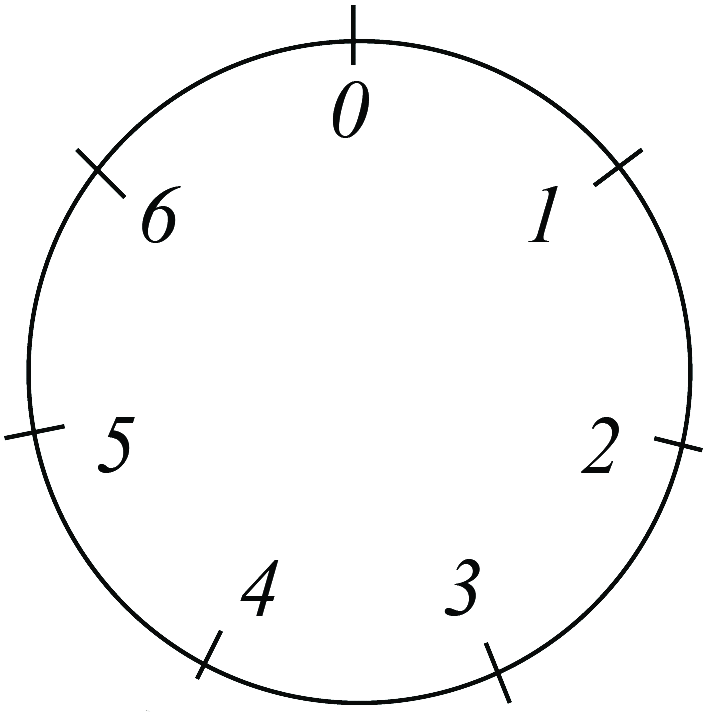
\includegraphics[width=0.2\linewidth]{img/aritmetica_modulare_mod7.png}
\end{center}
Comunque scielgo un numero $\in \mathbb{N}$ riesco a rappresentarlo tramite $n \text{ mod } 7$. Così facendo riduco l'aritmetica a 7 numeri. \\\\
Quando due numeri sono rappresentabili dalla stessa cifra? Quando il resto della divisione intera è uguale:
\[
	x\equiv y \Leftrightarrow x \text{ mod } n = y \text{ mod } n
\]
Quando $x-y$ è divisibile per $n$?
\begin{gather*}
	\begin{rcases*}
		x = q_1 \cdot n + r_1 \\
		y = q_2 \cdot n + r_1
	\end{rcases*} 0 \leq r < 7\\
	x-y = \underbracket{(q_1 - q_2)n}_{\text{divisibile per $n$}} + \cancel{(r_1-r_1)}
\end{gather*}

\subsection{Proprietà}
\textbf{Somma}
\begin{itemize}
	\item $x + (y+z) = (x+y) + z$
	\item $x+y=y+x$
	\item $x+(-x) = 0$ \qquad elemento opposto
	\item $x+0=x$ \qquad elemento neutro
\end{itemize}
La somma è un gruppo additivo che è commutativo\\\\
\textbf{Prodotto}
\begin{itemize}
	\item $x(yz) = (xy)z$
	\item $xy=yx$
	\item $x\cdot1 = x$ \qquad elemento neutro
	\item $x\cdot 0=0$
	\item $x\cdot x^{-1} = 1$ \qquad $\forall x \neq 0$ \qquad inverso
\end{itemize}
Gruppo moltiplicativo
\newpage
\noindent \textbf{Calcolo dell'inverso}:l'inverso si può calcolare solo quando il modulo è un numero primo, altrimenti, in caso di modulo non primo, gli unici numeri invertibili sono quelli primi fra loro con il modulo.\\
In modulo 7 per esempio:
\begin{gather*}
	2 \cdot 4 \equiv_7 1 \qquad \text{l'inverso del 2 è il 4, in aritmetica modulare mod 7}\\
	3 \cdot 5 \equiv_7 1\\
	6 \cdot 6 \equiv_7 1
\end{gather*}\\
Quando siamo in un aritmetica modulare modulo $n$, ed $n$ è un \underline{numero primo}, abbiamo un \underline{campo numerico}.

\subsection{Proprietà fondamentali del modulo}
Tre \textbf{proprietà fondamentali} nell'aritmetica modulare:\\\\
Presi du numeri interi $A$ e $B$:
\begin{gather*}
	(A+B) \mmod n = \big((A \mmod n) + (B \mmod n)\big) \mmod n \\
	(A\cdot B) \mmod n = \big((A \mmod n) \cdot (B \mmod n)\big) \mmod n \\
	A^k \mmod n = (A \mmod n)^k \mmod n
\end{gather*}
\subsubsection{Esempi di utilizzo}
Calcolare il modulo di numeri molto grandi
\begin{gather*}
	\begin{split}
		(125342\textcolor{red}{3} \cdot 13443\textcolor{red}{2}) \mmod 5 &= \\
		&= (3 \cdot 2) \mmod 5\\
		&= 6 \mmod 5 = 1
	\end{split}\\\\
	\begin{split}
		2^{99} \mmod 7 &= \\
		&= 2^{9\cdot 11} = (2^9)^11 \\
		&= (2^3\cdot 2^3 \cdot 2^3)^{11} = \\
		&= (1\cdot1\cdot1)^{11} \equiv_7 1
	\end{split}\\\\
	\begin{split}
		34^{217} \mmod 7 &= \\
		&= 37\equiv_7 -1 \\
		&= (-1)^{217} \equiv_7 -1 \equiv_7 6
	\end{split}\\\\
	3^{1227645} \mmod 12 \equiv 3 \qquad \text{perchè } 3^i \mmod 12 = 1,\underbracket{3,9}_{periodo},3,9,3,9 ...	
\end{gather*}
\subsection{Periodo}
L'operazione $a^b \mmod n$ è periodica a partire da un valore $h\leq n$ con periodo di un certo $t$.\\\\
Esempio in aritmetica modulo 7:
\[
	\underbracket{2^0 \equiv 1 \qquad 2^1\equiv2 \qquad 2^2\equiv4}_{\text{periodo}} \qquad 2^3 \equiv 1 \qquad 2^4 \equiv 2 \qquad 2^5\equiv4\qquad... \qquad t=3
\]
\[
	\underbracket{3^0 \equiv 1 \qquad 3^1\equiv3 \qquad 3^2\equiv2 \qquad 3^3\equiv6}_{\text{periodo}} \qquad 3^4\equiv1 \qquad 3^5\equiv3 \qquad... \qquad t=4
\]
\newpage
\noindent\textbf{Dimostrare il periodo}
\begin{gather*}
	a^1 \mmod n \qquad a^2 \mmod n \qquad ... \qquad a^{n+1} \mmod n\\
	\begin{rcases*}
		1 \leq h \leq n+1\\
		1\leq k \leq n+1
	\end{rcases*} a^h \mmod n = a^k \mmod n \\
	a^{h+1} \mmod n = a^{k+1} \mmod n \Rightarrow a^{h+i} \mmod n = a^{k+i} \mmod n \; \forall i
\end{gather*}

\subsection{MCD e teorema di Eulero}
\begin{gather*}
	\mcd{a}{b} \in \N \\
	\mcm{a}{b} \in \N
\end{gather*}
Come si calcolano MCD e mcm?
\begin{gather*}
	100 = 2^ \cdot 5^2 \qquad 46=2\cdot 23\\
	\mcd{100}{46} = 2\qquad \mcm{100}{46}=2^2\cdot 23 \cdot 5^2
\end{gather*}
\textbf{Teorema di Eulero}
\begin{gather*}
	\mcd{a}{b} = b \text{ se } b\;|\;a \text{ altrimenti}\\
	\text{se } b \not| \; a \text{ allora } \mcd{a}{b} = \mcd{b}{\text{resto}(a,b)}
\end{gather*}
Perché questo teorema è più efficiente?
\begin{gather*}
	\text{Dati due numeri $a$ e $b$, posso scrivere $a$ come}\\
	a = b\cdot q + r \qquad \text{con } 0<r<b\\
	\text{ora prendo un divisore comune di $a$ e $b$}:\\
	\text{se il divisore } |\; a \text{, allora divide anche } a-q\cdot b \quad(\text{ovvero il resto}) \\\\
	a=d\cdot s_1 \qquad b=d\cdot s_2\\
	r \to a - q\cdot b = d\cdot s_1 - d\cdot s_2 = \underbracket{d(s_1 - s_2)}_{\divides{d}{r}}\\\\
	\begin{split}
		a &= q\cdot b + r \\
		&= q(e\cdot t_1) + e\cdot t_2 \\
		&= \underbracket{e(q\cdot t_1 + t_2)}_{\divides{e}{a}}
	\end{split}
\end{gather*}
Regola generalizzata
\begin{gather*}
	a = b\cdot q_1 +r_1 \qquad \text{con }0\leq r_1 < b \\
	b = r_1 \cdot q_2 + r_2 \qquad \text{con }0\leq r_2 < r_1 \\
	r_1 = r_2 \cdot q_3 + r_3 \qquad \text{con }0\leq r_3 < r_2 \\
	r_2 = r_3 \cdot q_3 + r_4 \qquad \text{con }0\leq r_4 < r_3 \\
	r_{n-1} = r_n \cdot q_{n} + r_{n+1} \qquad \text{con } 0\leq r_{n+1}<r_{n-2}\\
	r_{n} = r_{n+1} \cdot q_{n+1} + \textcolor{red}{ r_{n+2}} \qquad \text{con } 0\leq r_{n+2}<r_{n+1} \\
\end{gather*}
Dove MCD è l'ultimo resto diverso da zero [$r_{n+2}$]

\newpage
\textbf{Esercizio}
\begin{gather*}
	\begin{align*}
		\mcd{1024}{666} &= \\
		1024 &= 1 \cdot 666 + 358 \\
		666 &= 1 \cdot 358 + 308\\
		358 &= 1\cdot 308 + 50 \\
		308 &= 6\cdot 50 + 8\\
		50 &= 6\cdot 8 + \textcolor{red}{2} \to \text{MCD}\\
		8 &= 4\cdot 2 + 0
	\end{align*}
\end{gather*}
Due numeri si dicono primi fra loro se il loro MCD è uguale a 1.

\subsection{Proprietà di Bezut}
Siano $a,b,c \neq 0$ allora l'equazione $ax + by = c$ ha soluzioni intere se $\mcd{a}{b}$ divide $c$.\\[2mm]
In particolare se \mcd{a}{b} = 1 allora l'equazione $ax + by = c$ ha soluzione per ogni $c$.\\\\
\textbf{Esempio}
\begin{gather*}
	120x + 8y = 12\\
	\mcd{120}{8} = 3 \qquad \text{quindi devo trovare una combinazione lineare che dia 3}\\
	\mcd{\frac{120}{3}}{\frac{81}{3}} = \frac{3}{3} \qquad \to \qquad  \mcd{40}{27} = 1\\\\
	\begin{split}
		40x+27y&=1\\
		-2\cdot 40 + 3\cdot 27 &= 1\\
		12\cdot(-2\cdot 40) + 12\cdot(3\cdot 27) &= 12 \cdot 1\\
		-960 + 972 &= 12\\
		-960 &= -960 \\
		0 &= 0 \checkmark
	\end{split} 
\end{gather*}
\textbf{Esempio}\\[2mm]
Trovare la combinazione lineare che soddisfi
\begin{gather*}
	7x+14y = 5\\\\
	5 \text{ non divide 7}\\
	\mcd{7}{14} = 7 \qquad \text{non ammette soluzioni intere}
\end{gather*}
\newpage
\subsection{Equivalenze}
\[ax \equiv_c b\]
\textbf{Esercizio}
\begin{gather*}
	3x \equiv_5 2\\
	\divides{5}{\underbracket{3x+2}_{\mathclap{\text{combinazione lineare di 3 e 2}}}}\\[1mm]
	\begin{split}
		3^{-1}\cdot 3x = 3^{-1}\cdot 2 \Rightarrow &\\
		& x = 3^{-1}\cdot 2 \\
		&x = 2\cdot 2 \\
		& x=4 \checkmark
	\end{split}
\end{gather*}
\textbf{Esercizio}
\begin{gather*}
	4x \equiv_{13} 11 \qquad \text{ 11 è un numero primo, forma un campo numerico. Tutti i numeri $\neq 0$ sono invertibili}\\
	\begin{split}
		x &= 4^{-1} \cdot 11 \\
		&= 10 \cdot 11 \quad \mmod 13\\
		&= 110 \mmod 13 \\
		&= 6
	\end{split}\\
	4\cdot 6 \equiv_{13} 11\\
	24 \equiv_{13} 11
\end{gather*}
\textbf{Esercizio}
\begin{gather*}
	2x \equiv_{15} 7 \qquad \text{ 15 non è un numero primo. Gli unici numeri invertibili sono quelli primi fra loro con il modulo} \\
	\begin{split}
		x &= 2^{-1} \cdot 7 \\
		&= 8 \cdot 7 \quad \mmod 15\\
		&= 56 \mmod 15 \\
		&= 11
	\end{split}\\
	2\cdot 11 \equiv_{15} 7\\
	22 \equiv_{15} 7 \checkmark
\end{gather*}

\newpage
\subsection{Congruenze lineari}
\begin{gather*}
	ax \equiv_n c \qquad (n \geq 2, a \not\equiv_n 0)\\
	\divides{n}{ax-c} \to ax-c=q\cdot n\\
	ax - q\cdot n = c \to \text{ 1 soluzione intera se } MCD(a,n) \;|\; c	
\end{gather*}
In una confruenza lineare, ci sono tante soluzioni quante $\mcd{a}{n}$
E\subsubsection{Esempio 1}
\begin{gather*}
	3x \equiv_{12} 6 \\
	MCD(3,6)=\divides{3}{6} \text{? Si, 1 soluzione intera, } \to x=2  
\end{gather*}
\subsubsection{Esempio 2}
\begin{gather*}
	224x \equiv_8 46 \\
	MCD(224,8)=\divides{8}{46} \text{? No, nessuna soluzione} 
\end{gather*}
\subsubsection{Esempio 3}
\begin{gather*}
	ax + by \\
	124x \equiv_{71} 17\\
	MCD(124,71) = 1 \;|\; 17 \text{? Si, 1 soluzione, ma quale?}\\
	x \equiv_{71} 124^{-1}\cdot 17 \qquad\qquad 124\equiv_{71} = 53\\
	x \equiv_{71} 53^{-1}\cdot 17 \text{ e cerco la soluzione ...}\\
	\text{oppure}\\
	\text{Controllo che 17 sia una combinazione lineare di 53 e 71:}\\
	53x + \underbracket{71y}_{\equiv_{71} 0} \equiv_{71} 17	\\
	53\cdot 3 + 71\cdot(-2) \equiv_{71} 17 \\
	x=3 \qquad y=-2
\end{gather*}
\subsubsection{Esempio 4}
\begin{gather*}
	7074x \equiv_{123} 865 \qquad 865 \equiv_{123} 4\\
	7074x \equiv_{123} 4 \qquad 7074 \equiv_{123} 63 \\
	\begin{split}
		63x \equiv_{123} 4 \to & \\
		& 123 = 3\cdot 41 \\
		& 63 = 3 \cdot 21 \\
		& MCD(123,63) = 3 \;|\; 4 \text{? No, nessuna soluzione}
	\end{split}
\end{gather*}


\newpage
\subsection{Teorema cinese del resto}
\begin{gather*}
	\text{Siano $n_1, \dots, n_k$ interi positivi a due a due primi fra loro}\\
	MCD(n_i, n_j)=1 \qquad \text{se } i\neq j\\
	x \equiv_{n_1} a_1 \\
	x \equiv_{n_2} a_2 \\
	\dots\\
	x \equiv_{n_k} a_k\\
	\text{ammette un unica soluzione minore di $n_1 \cdot n_2 \cdot ... \cdot n_k$}
\end{gather*}
\subsubsection{Esempio senza teorema cinese}
\begin{gather*}
	x \equiv_3 2 \qquad a\\
	x \equiv_5 3 \qquad b\\
	x \equiv_7 2 \qquad c\\
	\text{Il sistema ammette 1 unica soluzione $< 3\cdot5\cdot7 = 105$}\\
	\begin{rcases*}
		a: \qquad 2,5,8,11,...,2+3k\\
		b: \qquad 3,8,13,18,...,3+5s\\
		c: \qquad 2,9,16,23,...,2+7l
	\end{rcases*}
	\text{ prendo la soluzione in comune}\\
	\begin{rcases*}
	 a: \qquad 8,23,38,53,68,83,98,...\\
	 b: \qquad 23 ...\\
	 c: \qquad 23 ...
	\end{rcases*}
	\to 23 < 105\\
	\text{prova}\\
	N_r = n_1 \cdot n_2 \cdot ... \cdot n_{r-1} \cdot n_{r+1} \cdot ... \cdot n_k\\
	MCD(N_2, n_r) = 1 \to \text{sono primi fra loro}\\
	\overline{x} = a_1\cdot \underbracket{N_1 \cdot x_1}_{\equiv_{n_1} 1} + a_2\cdot N_2 \cdot x_2 + ... + a_k\cdot N_k \cdot x_k\\
	N_rx \equiv_{n_r} 1 \to \text{ esiste una soluzione} 
\end{gather*}
\begin{gather*}
	x \equiv_3 2 \qquad n_1 = 3 \qquad N_1 = 5\cdot 7 = 35\\
	x \equiv_5 3 \qquad n_2 = 5 \qquad N_2 = 3\cdot 7 = 21\\
	x \equiv_7 2 \qquad n_3 = 7 \qquad N_3 = 3\cdot 5 = 15\\\\
	MCD(n_1, N_1) = 1 \qquad \text{ primi fra loro}\\
	MCD(n_2, N_2) = 1 \qquad \text{ primi fra loro}\\
	MCD(n_3, N_3) = 1 \qquad \text{ primi fra loro}\\\\
	\begin{rcases*}
		N_1x_1 \equiv_{n_1} 1 \\
		N_2x_2 \equiv_{n_2} 1 \\
		N_3x_3 \equiv_{n_3} 1
	\end{rcases*}
	\to \text{ ammette una soluzione intera, } MCD(N_1\cdot x_1, n_1) = 1 \;|\; \checkmark\\\\
	35x_1 \equiv_3 1 \qquad 35\equiv_3 2 \qquad 2x_1 \equiv_3 1 \qquad x_1 \equiv_3 1\cdot2^{-1} \qquad x_1 \equiv_3 2\\
	21x_2 \equiv_5 1 \qquad 21 \equiv_5 1 \qquad x_2 \equiv_5 1\\
	15x_3 \equiv_7 1 \qquad 15 \equiv_7 1 \qquad x_3 \equiv_7 1\\\\
	\begin{split}
		\overline{x} &= (a_1\cdot N_1 \cdot x_1) + (a_2\cdot N_2 \cdot x_2) + (a_3\cdot N_3 \cdot x_3)\\
		&= 2\cdot 35 \cdot 2 + 3\cdot 21 \cdot 1 + 5\cdot 15 \cdot 1 \\
		&= 233 \equiv_{105} = 23 \;\checkmark
	\end{split}
\end{gather*}

\newpage
\subsection{Piccolo teorema di Fermat}
Se $p$ è un numero primo, e $p$ non divide $a$, allora 
\[ 
	a^{p-1} \equiv_p 1
\]
\textbf{Esempio:}
\begin{gather*}
	5^{6} \equiv_{7} 1 \\
	5^{30} \equiv_{31} 1 \\
	20^{30} \equiv_31 1
\end{gather*}
Se prendo i multipli di $a$ 
\[ 
	a,2a,3a,...,(p-1)a
\]
ovvero $ (p-1) $ multipli, deduco che
\[
	ka \not\equiv_p ra \qquad \text{con } 1 \leq k\neq r \leq(p-1)
\]
Se suppongo per assurdo che $ka \equiv_7 a ra$ sia vero. Se è vero allora
\begin{gather*}
	\divides{p}{ka-ra} = a(k-r)\\
	\text{da cui segue che} \\
	\underbracket{\divides{p}{k-r}}_{\text{impossibile}} \qquad \text{perché } (k-r) < p
\end{gather*}
Quindi
\[
	a \cdot 2a \cdot 3a \cdot ... \cdot (p-1)\cdot a \equiv_p (p-1)!
\]
\textbf{Esempio numerico:}
\begin{gather*}
	p=7 \qquad a=3\\
	\text{multipli di $a$:} \quad 3,6,2,5,1,4 \qquad \text{[tutti i numeri da 1 a 6 in disordine]}\\
	3\cdot 6\cdot 2\cdot 5\cdot 1\cdot 4 \equiv_7 6!\\
	a^{p-1} \cdot (p-1)! \mod{7}\Rightarrow a^{p-1} \equiv_7 1 \checkmark
\end{gather*}

\noindent\textbf{Esercizio:}
\[ 4^{253} \equiv_7 ? \]
Soluzione
\begin{gather*}
	4^{253} = 4^{6\cdot 42 + 1} = 4\cdot (4^{6})^{42} \equiv_7 4\cdot 1^{42} = 4
\end{gather*}

\newpage
\subsubsection{Teorema}
Se $p$ è un numero primo, allora $ a^{p} \equiv_p a $.\\[2mm]
\textbf{Dimostrazione}
\begin{gather*}
	\text{se } \divides{p}{a},\; a^{p} \equiv_p 0 \\
	\begin{split}
		\text{se } \notdivides{p}{a},\; a^{p-1} &\equiv_p 1 \\
		a\cdot a^{p-1} &\equiv_p a\\
		a^{p} &\equiv_p a
	\end{split}	
\end{gather*}
\textbf{Dimostrazione per induzione}
\[
	\text{Base: } a=0 \qquad \text{il teorema è ovvio} \checkmark \\
\]
Suppongo per induzione che $ a^{p} \equiv_p a $:
\begin{gather*}
	\begin{split}
		(a+1)^{p} &= a+1\\
		&= \sum_{i=0}^{p} \binom{p}{i}a^i \cdot 1^{p-1} = \binom{p}{0} + \underbracket{\cancel{\binom{p}{1}a}}_{\mathclap{\text{a lo divide}}} + \cancel{\binom{p}{2}a^2} + \dots + \cancel{\binom{p}{p-1}a^{p-1}} + \binom{p}{p}a^p\\
		& \text{sapendo che } \binom{p}{i} = \dfrac{p!}{i!(p-i)!} \qquad \binom{p}{0} = 1 \qquad \binom{p}{p} = 1 \qquad \text{deduco che}\\
		(a+1)^{p} &\equiv_p 1 + a^{p} \equiv_p 1 + a \checkmark
	\end{split}\\
\end{gather*}
\linea


\noindent
Se $p$ e $q$ sono numeri primi diversi, $a^{p} \equiv_p a$ e $ a^{q} \equiv_p a$, allora $a^{pq} \congruente{pq} a$.\\\\
\textbf{Esempio:}
\begin{gather*}
	p=11 \qquad q=31 \\
	2^{11} \congruente{31} 2\\
	2^{31} \congruente{11} 2
\end{gather*}

\subsection{Teorema di Eulero}
$\phi(n) = $ numero di elementi minori di $n$ che sono relativamente primi con $n$.\\
Es. $\phi(9) = 1,2,4,5,7,8 = 6$\\\\
Se $p$ è primo, allora $\phi(p^k) = p^k - p^{k-1} = p^k \cdot (1 - \dfrac{1}{p})$\\\\
Se $a$ e $n$ sono primi fra loro, $a^{\phi(n)} \congruente{n} 1$\\\\
La funzione di Eulero è moltiplicativa:
\[
	\phi(nk) = \phi(n)\cdot \phi(k) \qquad \text{se $n$ e $k$ sono primi fra loro}
\]
Esempio: 
\begin{gather*}
	\phi(9) = \phi(3^2) = 3^2 - 3 = 6\\
	\phi(100) = \phi(4\cdot25) = \phi(2^2\cdot 5^2) = \phi(2^2)\cdot\phi(5^2) = (2^2-2)(5^2 - 5) = 2 \cdot
\end{gather*}

\newpage
\subsection{Esercizi}
\subsubsection{Esercizio 1}
Determinare $12^{26} \congruente{13}$
\begin{gather*}
	12 \congruente{13} -1 \\\\
	\begin{split}
		12^{26} &\congruente{13} (-1)^{26} \\
		&\congruente{13} 1
	\end{split}
\end{gather*}


\subsubsection{Esercizio 2}
Determinare le soluzioni di $2x \congruente{4} 3$
\begin{gather*}
	\mcd{2}{4} = \divides{2}{3} \text{? No, nessuna soluzione}
\end{gather*}


\subsubsection{Esercizio 3}
Determinare le soluzioni di $3x \congruente{4} 2$. Le soluzioni sono $x=2 + 4k, k\in \ins{Z}$ 

\subsubsection{Esercizio 4}
Determinare le soluzioni di $6x \congruente{4} 2$. Le soluzioni sono $x12 + 4k, k\in \ins{Z}$ 

\subsubsection{Esercizio 5}
Determinare le soluzioni di $3x \congruente{4} 2$. Le soluzioni sono $x=2 + 4k, k\in \ins{Z}$ 

\subsection{Tutorato}
\subsubsection{Esercizio 1}
Determinare $-1027$ \congruente{16} ?
\begin{gather*}
	\begin{split}
		-1027 &= -1(1024 + 3)\\
		&= -1(2^{10} + 3) \\
		&= -1(2^{4+6}+3)\\
		&= -1(16\cdot2^{6} + 3) \\
		&= -1(0+3) \\
		&= -3 \\
		& = 13 \mmod 16
	\end{split}
\end{gather*}
\begin{gather*}
	\begin{split}
		(-1027)^{17} &\congruente{16} (-3)^{17} \\
		&\congruente{16} (-3)^{4+4+4+4+1} \\
		&\congruente{16} (-3)^{4\cdot 4 + 1} \\
		&\congruente{16} ((-3)^4)^4 \cdot (-3)^1\\
		&\congruente{16} (81)^4\cdot(-3) \\
		&\congruente{16} 1^4 \cdot (-3) \\
		&\congruente{16} -3 \\
		&\congruente{16} 13
	\end{split}
\end{gather*}

\subsubsection{Esercizio 2}
Determinare $19693^{12}$ \congruente{7} ?
\begin{gather*}
	\begin{split}
		19693^{12} &\congruente{7} (14770 + 4923)^{12} \\
		&\congruente{7} 4923^{12} \\
		&\congruente{7} (4921 + 2)^{12} \\
		&\congruente{7} 2^{12} \\
		&\congruente{7} 2^{3\cdot 4} \\
		&\congruente{7} (2^3)^4 \\
		&\congruente{7} (1)^4 \\
		&\congruente{7} 1
	\end{split}
\end{gather*}

\subsubsection{Esercizio 3}
Determinare $243^{270}$ \congruente{8} ?
\begin{gather*}
	\begin{split}
		243 &\congruente{8} (240 + 3)^{270} \\
		&\congruente{8} 3^{270} \\
		&\congruente{8} 3^2 \cdot 3^{268} \\
		&\congruente{8} (3^2)^{268} \\
		&\congruente{8} (1)^{268} \\
		&\congruente{8} 1
	\end{split}
\end{gather*}

\subsubsection{Esercizio 4}
Determinare $172!$ \congruente{330} ?\\[2mm]
Dato che il fattoriale si compone come
\[
	172\cdot 171 \cdot ... \cdot 33 \cdot ... \cdot 10 ... \cdot 1
\]
sarà sicuramente divisibile per 330, e quindi
\[
	172! \congruente{330} 0
\]

\subsubsection{Esercizio 4}
Determinare $215^{26}$ \congruente{13} ?
\begin{gather*}
	\begin{split}
		215^{26} \congruente{13}& 7^{26} \\
		\congruente{13}& 7^{12+14} \\
		\congruente{13}& 1\cdot 7^{12} \cdot 7^2 \qquad \text{piccolo teorema di Fermat}\\
		\congruente{13}& 1\cdot 1 \cdot 49 \mmod 13 \\
		\congruente{13}& 10
	\end{split}
\end{gather*}

\subsubsection{Esercizio 6}
Determinare $512^{99}$ \congruente{11} ?
\begin{gather*}
\begin{split}
512^{99} &\congruente{11} (512^{11})^ 9 \\
	&\congruente{11} \left((2^9)^{11}\right)^9 \\
	&\congruente{11} (2^9)^9 \qquad \text{teorema di Fermat}\\
	&\congruente{11} 2^{81} \\
	&\congruente{11} 2^{80 + 1} \\
	&\congruente{11} 2^{8\cdot 10 + 1} \\
	&\congruente{11} (2^{10})^8 \cdot 2 \\
	&\congruente{11} 1^8 \cdot 2 \qquad \text{piccolo teorema di Fermat} \\
	&\congruente{11} 2
\end{split}
\end{gather*}

\newpage
\section{Relazioni}
\tright{17-11-2015}
Una relazione $R$ di dominio $A$ e codominio $A$ è un sottoinsieme di $A\times A$:
\[
	R \subseteq A \times A
\]
Le relazioni si dividono in due fasce:
\begin{itemize}
	\item relazione di \textbf{ordinamento parziale}
	\item relazione di \textbf{equivalenza}
\end{itemize}
\subsection{Relazione di ordinamento parziale}
\begin{enumerate}
	\item \textbf{proprietà riflessiva}: ogni elemento è in relazione con se stesso
		\[
			\forall x(xRx)
		\]
	\item \textbf{proprietà transitiva}: se $x$ è in relazione con $y$ e $y$ è in relazione con $z$ allora $x$ è in relazione con $z$
		\[
			\forall xyz (xRy \land yRz \to xRz)
		\]  
	\item \textbf{proprietà antisimmetrica}: se $x$ è in relazione con $y$ e $y$ è in relazione con $x$ allora $x=y$
		\[
			\forall xy (xRy \land yRx \to x=y)
		\]
\end{enumerate}
	
\subsection{Relazione di equivalenza}
\begin{enumerate}
	\item \textbf{proprietà riflessiva}: ogni elemento è in relazione con se stesso
		\[
			\forall x(xRx)
		\]
	\item \textbf{proprietà transitiva}: se $x$ è in relazione con $y$ e $y$ è in relazione con $z$ allora $x$ è in relazione con $z$
		\[
			\forall xyz (xRy \land yRz \to xRz)
		\]  
	\item \textbf{proprietà simmetrica}: se $x$ è in relazione con $y$ e $y$ allora $y$ è in relazione con $x$
		\[
			\forall xy (xRy \to yRx)
		\]
\end{enumerate}
Da notare che la \underline{proprietà riflessiva}, comune ad entrambe le fasce,  \underline{non vale nel sottoinsieme ristretto}
\begin{gather*}
	2 \leq 2 \text{ ha la proprietà riflessiva? } \checkmark\\
	2 < 2 \text{ ha la proprietà riflessiva? } \crossmark
\end{gather*}


\newpage
\subsection{Esempi}
\subsubsection{Esercizio 1}
Verifichiamo quali proprietà valgono in
\[
	xRy \text{ sse } x+y=5 \qquad \text{con } x,y \in \ins{N}
\]
\begin{itemize}
	\item proprietà riflessiva:
	\begin{gather*}
		\begin{split}
			\forall x \in \ins{N}(xRx) \to \; & x+ x = 5 \\
			& 2x = 5 \\
			\textit{controesempio:}\quad & 2\cdot 10 = 5 \crossmark
		\end{split}
	\end{gather*}
	
	\item proprietà transitiva: 
		\begin{gather*}
			\begin{cases*}
				x + y = 5 \\
				x + z = 5
			\end{cases*}
			\quad \text{ implica }  x+z = 5 \\\\
			\textit{controesempio: } x=2,\; y=3,\; z=2 \\
			x + y = 2 + 3 = 5 \\
			y + z = 3 + 2 = 5 \\
			x + z = 2 + 2 = 5 \crossmark
		\end{gather*}
	\item proprietà simmetrica:
		\[
			x + y = 5 \to y + x = 5 \checkmark
		\] 
	\item proprietà antisimmetrica:
		\begin{gather*}
			x=3, \; y=2 \\[2mm]
			\begin{cases*}
				3 + 2 = 5 \\
				2 + 3 = 5
			\end{cases*}
			\quad \to 2=5 \crossmark
		\end{gather*}
\end{itemize}

\subsubsection{Esercizio 2}
Verifichiamo quali proprietà valgono in
\[
	xRy \text{ sse } x \text{ e } y \text{ hanno la stessa altezza} \qquad \text{con }x,y \in \{\text{aula 1}\}
\]
\begin{itemize}
	\item proprietà riflessiva: \checkmark
	\item proprietà transitiva: \checkmark
	\item proprietà simmetrica: \checkmark
	\item proprietà antisimmetrica: \crossmark
\end{itemize}
Questa relazione è una \underline{relazione di equivalenza }, in quanto vengono soddisfatte tutte le proprietà necessarie.

\newpage
\subsubsection{Esercizio 3}
Verifichiamo quali proprietà valgono in
\[
	xRy \text{ sse } x \congruente{5} y \qquad \text{con } x,y \in \ins{Z}
\]
\begin{itemize}
	\item proprietà riflessiva: 
		\begin{gather*}
			x \congruente{5} x \text{ ?}\\
			\divides{5}{(x-x)} \checkmark
		\end{gather*}
	\item proprietà transitiva: 
		\begin{itemize}
			\item $\divides{5}{x-y}$
			\item $\divides{5}{y-z}$
				\begin{gather*}
					x-y = 5\cdot k \qquad \text{per un certo $k$} \\
					y-z = 5\cdot r \qquad \text{per un certo $r$} \\
					(x-y) + (y-z) = 5k + 5r \\
					\divides{5}{x-z} = 5(k+r) \checkmark
				\end{gather*}
		\end{itemize}
	\item proprietà simmetrica: 
		\begin{gather*}
			x\congruente{5} y \to y \congruente{5} x \\
			\divides{5}{x-y} \to x-y = 5\cdot k \qquad \text{per un certo $k$}\\
			\divides{5}{y-x} \to y-x = -5\cdot k \qquad \text{per un certo $k$} \checkmark
		\end{gather*}
	\item proprietà antisimmetrica: se vale la proprietà simmetrica, non può valere anche quella antisimmetrica.
\end{itemize}
Questa è una relazione di equivalenza a 5 classi.

\subsubsection{Esercizio 4}
Sia \ins{N} l'insieme dei numeri naturali. $\ins{N}^2 = \ins{N} \times \ins{N}$
\begin{gather*}
	R \subseteq \ins{N}^2 \times \ins{N}^2\\
	(a,b)R(c,d) \text{ sse } a+b+3=c+d+1
\end{gather*}
Verifico quali proprietà possiede
\begin{itemize}
	\item riflessiva: $\forall(x,y) \quad (x,y)R(x,y)$
		\[
			x+y+3 = x + y + 1 \crossmark
		\]
	\item irriflessiva: $\forall(x,y) \quad \lnot\left[(x,y)R(x,y)\right]$
		\[
			x+y+3 \neq x + y + 1 \checkmark
		\]	
	\item simmetrica: $\forall(x,y) \quad (x,y)R(a,b) \to (a,b)R(x,y)$
		\begin{gather*}
			a+b+3 = c+d+1 \\
			c+d+3=a+b+1 \\\\
			c+d+3= (c+d+1)+2 = (a+b+3)+2 = a+b+5 \neq a+b+1 \crossmark
		\end{gather*}
	\item transitiva: $(a,b)R(c,d) \land (c,d)R(e,f) \to (a,b)R(e,f)$
		\begin{gather*}
			a+b+3 = c+d+1 \quad\land\quad c+d+3=e+f+1 \quad\to\quad a+b+3=e+f+1\\\\
			a+b+3=c+d+1 = (c+d+3)-2 = (e+f+1) - 2 = e + f -1 \crossmark
		\end{gather*}
	\item antisimmetrica:  $(a,b)R(c,d) \land (c,d)R(a,b) \to (a,b)=(c,d)$
		\begin{gather*}
				a+b+3=c+d+1 \to (a+b)-(c+d)=-2\\
				c+d+3=a+b+1 \to (a+b)-(c+d)=2\\\\
				\text{l'ipotesi dell'implicazione è falsa, proprietà verificata} \checkmark
		\end{gather*}
\end{itemize}


\subsection{Teorema}
Sia $R \subseteq A \times A$ una relazione di equivalenza, allora se $a \in A$:
\[
	[a]_{_R} = \{ b \in A : aRb \}
\]
Questa notazione indica una classe di equivalenza, ovvero il sottoinsieme di tutti gli elementi equivalenti ad $a$. \\
Una notazione equivalente è $\nicefrac{a}{_R} = \{ b \in A : aRb \}$ 

\subsection{Partizioni}
Una partizione di $A$ è una famiglia di insiemi $\{ A_i \} \; i \in \overbracket{I}^{\mathclap{\text{indici}}}$ tali che
\begin{itemize}
	\item $A = \underset{i\in I}{U}  A_i$ 
	\item Ogni coppia $A_i, A_j$ con $i\neq j$
		\[
			A_i \cap A_j = \varnothing
		\]
\end{itemize}

\newpage
\subsubsection{Esempi}
\paragraph{Esempio 1}
\begin{gather*}
	A = \{ 1,2, ..., 16 \} \\
	I = \{ a,b,c \} 
\end{gather*}
Ogni indice deve essere associato ad un sottoinsieme di $A$.
\linea
Verificare che questa suddivisione sia una partizione di $A$:
\begin{gather*}
	A_a = \{ 2,7,8,11,15,16 \} \\
	A_b = \{ 1,3,5 \} \\
	A_c = \{ 4,9,10 \}
\end{gather*}
Controllo le intersezioni:
\begin{gather*}
	A_a \cap A_b = \varnothing \\
	A_a \cap A_c = \varnothing \\
	A_b \cap A_c = \varnothing \\\\
	A_a \cup A_b \cup A_c \subsetneq A \crossmark
\end{gather*}
In quanto l'unione delle partizioni dovrebbe darmi l'insieme di partenza, questa suddivisione non è una partizione. Possiamo notare infatti che all'unione mancano gli elementi $\{ 5,6,12,13,14 \}$.
\linea
Verificare che questa suddivisione sia una partizione di $A$:
\begin{gather*}
	A_a = \{ n \in A : n=0 \mmod 3 \} = \{ 3,6,9,12,15 \}\\
	A_b = \{ n \in A : n=1 \mmod 3 \} = \{ 1,4,7,10,13,16 \}\\
	A_c = \{ n \in A : n=2 \mmod 3 \} = \{ 2,8,11,14 \}
\end{gather*}
Controllo le intersezioni:
\begin{gather*}
	A_a \cap A_b = \varnothing \\
	A_a \cap A_c = \varnothing \\
	A_b \cap A_c = \varnothing \\\\
	A_a \cup A_b \cup A_c \subseteq A \checkmark
\end{gather*}
L'unione delle partizioni è uguale all'insieme di partenza, quindi questa suddivisione è una partizione.

\paragraph{Esempio 2}
\begin{gather*}
	x \congruente{7} y \\
	I = \{ 0,1,2,3,4,5,6 \} \qquad \text{insieme degli indici}\\
	Z_i = \{ n \in Z : n \congruente{7} i \} \qquad \text{partizioni} \\
	\underbracket{\underset{i = 0}{\overset{6}{U}}}_{\mathrlap{\text{unione di tutte le partizioni}}} Z_i = Z \qquad  \checkmark 
\end{gather*}

\subsection{Lemma}
Ogni partizione definisce una relazione di equivalenza, e viceversa:
\[
xRy \text{ sse } x,y \in A \land \exists i\in I (x,y \in A_i)
\]
Se $x$ e $y$ si trovano nello stesso inseme di una partizione, sono equivalenti.

\subsection{Esercizi}
\subsubsection{Esercizio 1}
Verificare quali proprietà ha la relazione:
\[
	(a,b)R(c,d) \Leftrightarrow \dfrac{3^a\cdot5^b}{3^c\cdot5^d} \leq 1
\]
\textbf{Inizio soluzione:} \\[2mm]
Prendo due coppie a caso e provo a sviluppare:
\[
	(5,7)R(1,2)\;?\qquad \dfrac{3^5\cdot5^7}{3^1\cdot 5^2} \leq 1 \qquad \crossmark
\]
controllo con un altra coppia:
\[
	(1,2)R(5,7)\;?\qquad \dfrac{3^1\cdot5^2}{3^5\cdot 5^7} \leq 1 \qquad \checkmark
\]
Dato che ho preso due coppie invertite, possiamo già ricavare che la relazione non è simmetrica (questo è un controesempio). Controllo le restanti proprietà:
\begin{itemize}
	\item riflessiva: $\forall x(xRx)$ dove $x=(a,b)$
		\[
				\dfrac{3^a\cdot5^b}{3^a\cdot 5^b} \leq 1 \qquad \checkmark	
		\]
	\item transitiva: $\forall xyz(xRy \land yRz \to xRz)$
		\[
			\dfrac{3^a\cdot5^b}{3^c\cdot 5^d} \leq 1 \quad\land\quad \dfrac{3^c\cdot5^d}{3^e\cdot 5^f} \leq 1 \to \left(\dfrac{3^a\cdot5^b}{\cancel{3^c\cdot 5^d}} \cdot \dfrac{\cancel{3^c\cdot 5^d}}{3^e\cdot 5^f}\right) \leq 1 \checkmark
		\]
		perché due numeri minori di 1 moltiplicati fra loro sono sempre minori di 1.
	\item antisimmetrica: $\forall xy(xRy \land yRx \to x=y)$
		\begin{gather*}
			\dfrac{3^a\cdot5^b}{3^c\cdot 5^d} \leq 1 \quad\Rightarrow\quad 3^a\cdot5^b\leq3^c\cdot5^d \\[2mm]
			\dfrac{3^c\cdot5^d}{3^a\cdot 5^b} \leq 1 \quad\Rightarrow\quad 3^c\cdot5^d\leq3^a\cdot5^b
		\end{gather*}
		queste due condizioni implicano $3^a\cdot5^b = 3^c\cdot 5^d$, da cui $a=c$ e $b=d$ \checkmark
\end{itemize}
Dato che la relazione gode di queste proprietà è un'ordinamento parziale di coppie di numeri naturali. Controllando viene verificata anche la proprietà totale (o una coppia è minore uguale ad un altra o viceversa), quindi la relazione è un ordinamento totale su $\ins{N}^2$

\subsubsection{Esercizio 2}
Quante funzioni iniettive e suriettive abbiamo da
\[
	\ins{N} \longmapsto \{0,1,2\}
\]
\begin{itemize}
	\item iniettive: 0, perché la cardinalità di \ins{N} è maggiore di quella del codominio	
	\item suriettive: $\infty$ 
\end{itemize}
Quante funzioni iniettive e suriettive abbiamo invece da
\[
	\{a,b\} \longmapsto \{ 0,1,2 \}
\]
\begin{itemize}
	\item suriettive: 0, perché la cardinalità del dominio non basta a coprire quella del codominio
	\item iniettive: $2\cdot 3 = 6$ funzioni iniettive
	\item non iniettive: 3, quando entrami i valori del dominio coprono lo stesso del codominio
\end{itemize}

\newpage
\subsection{Tutorato}
\subsubsection{Proprietà delle relazioni}
\begin{table}[h]
	\centering
	\begin{tabular}{c|ccc}
		\textbf{\begin{tabular}[c]{@{}c@{}}relazioni di\\ equivalenza\end{tabular}} & \multicolumn{3}{c|}{\textbf{relazioni di ordinamento}}                   \\ \hline
		& \textit{parziale} & \textit{stretto} & \textit{totale} \\ \cline{2-4} 
		riflessiva                                                                  & riflessiva        & irriflessiva     & riflessiva      \\
		simmetrica                                                                  & anti-simmetrica   & anti-simmetrica  & anti-simmetrica \\
		transitiva                                                                  & transitiva        & transitiva       & transitiva     
	\end{tabular}
\end{table}

\noindent La relazione totale è determinata come: \[\forall xy (xRy \lor yRx)\] mentre la relazione irriflessiva \[ \forall x (\lnot xRx) \]

\subsubsection{Classi di equivalenza}
Se $R$ è una relazioni di equivalenza nell'insieme $A$, $A$ può essere partizionato in più insiemi (almeno 1) in modo che tutti gli elementi di una partizione sono in relazione tra loro e non sono in relazione con gli elementi delle altre partizioni.

\subsubsection{Esercizi}

\paragraph{Esercizio 1}
Verificare di quali proprietà gode $\forall xy \in \ins{Z} \quad xRy \quad \text{sse } x+y \text{ è pari}$
\begin{itemize}
	\item proprietà riflessiva
		\[
			x + x \text{ è pari} = 2x \text{ è pari} \checkmark
		\]
	\item proprietà transitiva
		\begin{gather*}
			x + y = 2k \\
			y+z = 2r \\\\
			\begin{split}
				x+z &= (2k - y) + (2r - y) \\
				&= 2k + 2r - 2y \\
				&= 2(k+2 - y) \text{ sempre pari} \checkmark
			\end{split}
		\end{gather*}
\end{itemize}

\paragraph{Esercizio 2}
Determinare di quali proprietà gode la relazione
\[
	R: \qquad xRy \text{ sse } x^2 + y \geq 0 \qquad \forall xy \in \ins{Z}
\]
Inizio soluzione
\begin{itemize}
	\item proprietà riflessiva: $\forall x(xRx)$
		\begin{gather*}
			\text{due casi}
			\begin{cases*}
				x \geq 0 \to x^2 + x = x(x+1) \geq 0 \text{ vero perché } x\geq 0 \land x+1 \geq 1 \checkmark\\
				x \leq 0 \to x^2 + x = x(x+1) \leq 0 \text{ vero perché } x\leq 0 \land x+1 \leq 1 \checkmark
			\end{cases*}
		\end{gather*}
	\item irriflessiva: $\forall x \lnot(xRx)$. E' già riflessiva, non può essere irriflessiva
	\item simmetrica: $\forall xy (xRy \to yRx)$
		\begin{gather*}
			\text{è equivalente dire che } \exists xy \in \ins{Z} \; xRy \land \lnot(yRx)\\
			\text{trovo un controesempio:}\\
			x^2 + y = (-2)^2 + 1 = 4 + 1 \geq 0 \qquad xRy\\
			y^2 + x = 1^2 - 2 = \underset{\text{falso}}{-1 \geq 0} \qquad \lnot(xRy) \crossmark
		\end{gather*}
	\item antisimmetrica: $\forall xy (xRy \land yRx \to x=y)$
		\begin{gather*}
			\text{trovo un controesempio: } \\
			x=2 \qquad y=1\\
			x^2 + y = 2^2 + 1 = 5 \geq 0\\
			y^2 + x = 1^2 + 2 = 3 \geq 0\\
			5\neq 3 \to x\neq y \crossmark
		\end{gather*}
	\item transitiva: $\forall xyz (xRy \land yRz \to xRz)$
		\begin{gather*}
			\text{trovo un controesempio: } \\
			x=2 \qquad y=-4 \qquad z=-16\\
			x^2 + y = 2^2 - 4 = 0 \geq 0 \qquad xRy\\
			y^2 + z = (-4)^2 - 16 = 0 \geq 0 \qquad yRz \\
			x^2 + z = 2^2 - 16 = \underset{\text{falso}}{-12 \geq 0} \qquad \lnot(xRz) \crossmark\\
		\end{gather*}
	\item totale: $\forall xy (xRy \lor yRx)$
		\begin{gather*}
			\text{la relazione totale può essere scritta anche } \forall xy \lnot(xRy) \to xRy \\\\
			\text{suppongo che } \lnot(xRy) \Leftrightarrow \lnot(x^2 + y \geq 0) \Leftrightarrow x^2 + y < 0\\
			\text{allora}\\
			\begin{split}
				y &= -x^2 \\
				&= -x^2 - k \qquad k>0\\
				y^2 + x&= (-x^2 - k)^2 + x \\
				&> (-x^2)^2 + x \\
				&= x^4 + x \\
				&\geq x^2 + x \\
				&\geq 0 \qquad yRx
			\end{split}\\
			\textit{cazzo è sta roba?!}
		\end{gather*}
\end{itemize}
\newpage
\rtext{18-11-2015}
\section{Combinatoria}
\subsection{Principio moltiplicativo}
Se un elemento $x$ viene scelto tra $m$ elementi ed un elemento $y$ viene scelto tra $k$ elementi, allora le possibili scelte di $x$ e $y$ sono $m\cdot k$
\begin{gather*}
	x_1 \; ... \; m_1 \quad \text{scelte} \\
	\vdots \\
	x_r \; ... \; m_r \quad \text{scelte}
\end{gather*}
le scelte possibili sono quindi
\[
	\prod_{i=1}^{r} m_i
\]
\subsubsection{Esempi}
\paragraph{Esempio 1}
\[
	A = \{ a,b,c,d,e \}
\]
quante sono le possibili combinazioni di lunghezza 2?
\[
	\underbracket{5}\cdot \underbracket{5} = 25
\]
\paragraph{Esempio 2}
\[
	A = \{ 0,1,...,9 \}
\]
quante sono i numeri di lunghezza 6?
\[
	\underbracket{\;9\;} \cdot \underbracket{10}\cdot \underbracket{10}\cdot \underbracket{10}\cdot \underbracket{10}\cdot \underbracket{10} = 9\cdot 10^5
\]
perché nessun numero comincia con lo zero, la prima cifra varia da 1 a 9

\subsection{Principio additivo}
\subsubsection{Esempi}
\paragraph{Esempio 1}
se $|A| = k$ e $|B| = n$, quanto vale $|A\cup B|$?
\begin{gather*}
	\text{se } A \cap B = \varnothing \text{ allora } |A\cup B| = k + n \\
	\text{se } A \cap B \neq \varnothing \text{ allora } |A\cup B| = (k + n) - |A \cap B| \\
\end{gather*}
Ma questo caso si applica solo con due insiemi. Se avessimo più insiemi?
\paragraph{Esempio 2}
Regola a 3 insiemi:
\[
	|A\cup B \cup C| = |A \cup B \cup C| - |A \cap B| - |A \cap C| - |B \cap C| + |A \cap B \cap C|
\]
Prova numerica:
\begin{gather*}
	A = \{ a,b,c,d,e \} \\
	B = \{ c,e,f,g \} \\
	C = \{ a,b,c,f,h \} \\\\
	|A\cup B \cup C| = 14 - 2 - 3 - 2 + 1 = 8 \checkmark
\end{gather*}
\subsubsection{Regola generale}
Si deduce quindi che la regola generale per determinare la cardinalità dell'unione di più insiemi è:
\[
	|A_1 \cup A_2 \cup ... \cap A_n| = |A_1| + |A_2| + ... + |A_n| - \sum_{i\neq j}^{}\left( |A_i \cap A_j| \right)
\]

\subsubsection{Esempio complesso}
Quante sono le targhe in cui compare solo una lettera 'A'?
\[
	\underbracket{1} \underbracket{2} \quad \underbracket{3} \underbracket{4} \underbracket{5} \quad \underbracket{6} \underbracket{7}
\]
Nelle targhe italiane le targhe sono formate da 2 numeri, 3 lettere e due numeri:
\begin{gather*}
	X_1 = \text{insieme delle targhe con la 'A' in posto 1} \\
	X_2 = \text{insieme delle targhe con la 'A' in posto 2} \\
	X_6 = \text{insieme delle targhe con la 'A' in posto 6} \\
	X_7 = \text{insieme delle targhe con la 'A' in posto 7}
\end{gather*}
Quindi l'insieme delle targhe italiane con almeno una 'A' è determinato da
\begin{gather*}
		\begin{split}
			|X_1 \cup X_2 \cup X_6 \cup X_7| = &\quad |X_1| + |X_2| + |X_6| + |X_7| \\
			& - |X_1 \cap X_2| - |X_1 \cap X_6| - |X_1 \cap X_7| \\
			& - |X_2 \cap X_6| - |X_2 \cap X_7| \\
			& - |X_6 \cap X_7| \\
			& - |X_1 \cap X_2 \cap X_6 \cap X_7| \\
			& + |X_1 \cap X_6 \cap X_7| \\
			& + |X_1 \cap X_2 \cap X_6| \\
			& + |X_1 \cap X_2 \cap X_7| \\
			& + |X_2 \cap X_6 \cap X_7| \\\\
			&= 4 \cdot 26^3 \cdot 10^3 \text{ targhe con almeno una 'A'}
		\end{split}
\end{gather*}
Le targhe con esattamente una 'A' sono: $4\cdot 25^3 \cdot 10^3$ \\[2mm]
Le targhe che non hanno alcuna 'A' sono: $25^4 \cdot 10^3$ \\[2mm]
Le targhe che non hanno alcun '7' sono: $26^4 \cdot 9^3$ \\[2mm]
Le targhe che hanno solo una 'A' e solo un '7' sono: 
\[
	\underbracket{26^4 \cdot 10^3}_{\mathclap{\text{totali}}} - \overbracket{25^4\cdot 10^3}^{\mathclap{\text{senza 'A'}}} - \underbracket{26^4\cdot 9^3}_{\mathclap{\text{senza '7'}}} + \overbracket{25^4\cdot9^3}^{\mathclap{\text{senza 'A' e senza '7'}}} = 17'981'121
\]

\newpage
\subsubsection{Figure combinatorie}
\begin{table}[h]
	\centering
	\begin{tabular}{cc}
		\textbf{Disordine}                                                                           & \textbf{Ordine}                                                                             \\ \hline
		\multicolumn{1}{|c|}{\begin{tabular}[c]{@{}c@{}}combinazioni\\ semplici\end{tabular}}        & \multicolumn{1}{c|}{\begin{tabular}[c]{@{}c@{}}disposizioni \\ semplici\end{tabular}}       \\ \hline
		\multicolumn{1}{|c|}{\begin{tabular}[c]{@{}c@{}}combinazioni\\ con ripetizioni\end{tabular}} & \multicolumn{1}{c|}{\begin{tabular}[c]{@{}c@{}}disposizioni\\ con ripetizioni\end{tabular}} \\ \hline
	\end{tabular}
\end{table}


\paragraph{Disposizioni semplici}

\subparagraph{Esempio 1} dato un insieme $A$ di $n$ elementi, i posti a disposizione sono
\begin{gather*}
	\underbracket{\quad1\quad}\underbracket{\quad2\quad}\;...\;\underbracket{\quad k\quad}\\\\
	\disps{n}{k} = n(n-1)(n-2)...(n-k+1) = n!
\end{gather*}

\subparagraph{Esempio 2} dato un insieme $A=\{ a_1,a_2,...,a_n \}$ , le stringhe su $A$ si lunghezza $k$ senza ripetizioni di caratteri sono
\[
	\disps{n}{k} \qquad \text{con } k \leq n
\]

\paragraph{Disposizioni con ripetizioni}

\subparagraph{Esempio 1} dati gli insiemi $A = \{ a_1,...a_n \}$ e $A = \{ b_1,...b_k \}$, il numero di funzioni non iniettive da $B \longmapsto A$ sono
\begin{gather*}
	\begin{rcases*}
		b_1 \longmapsto a_1 \\
		b_2 \longmapsto a_2 \\
		\vdots \\
		b_k \longmapsto a_n
	\end{rcases*}
	\dispr{n}{k} = n^k
\end{gather*}


\paragraph{Combinazioni semplici}
Sia $A$ un insieme di $n$ elementi. Sia $k \leq n$. Una combinazioni semplice di ordine k di un insieme $A$ di $n$ elementi è un sottoinsieme di $A$ di cardinalità $k$.
\subparagraph{Esempio 1} l'insieme delle parti di un insieme è un esempio:
\[
	A = \{ a,b,c,d \} \qquad |A| = 4 \qquad |\mathcal{P}(A)| = ? 	 
\]
\begin{table}[h]
	\centering
	\begin{tabular}{ccccccll}
		&     & \multicolumn{2}{c}{$\varnothing$}    &     &    &  & \textbf{1} \\[3mm]
		& $\{ a \}$   & $\{ b \}$           & $\{ c \}$          & $\{ d \}$   &    &  & \textbf{4} \\[3mm]
		$\{ a,b \}$ & $\{ a,c \}$  & $\{ a,d \}$          & $\{ bd \}$         & $\{ c,d \}$  & $\{ b,c \}$ &  & \textbf{6} \\[3mm]
		& $\{ a,b,c \}$ & $\{ a,b,d \}$         & $\{ b,c,d \}$        & $\{ a,c,d \}$ &    &  & \textbf{4} \\[3mm]
		&     & \multicolumn{2}{c}{$\{ a,b,c,d \}$} &     &    &  & \textbf{1}
	\end{tabular}
\end{table}
\begin{gather*}
	|\mathcal{P}(A)| = \sum_{k=0}^{n} \binom{n}{k} = \sum_{k=0}^{4}\binom{4}{k} = 2^4 = 16\\\\
	\combs{n}{k} = \frac{\disps{n}{k}}{k!} = \frac{n!}{(n-k)!\cdot k!} = \binom{n}{k} \\
	\binom{n}{k} = \binom{n-1}{k-1} + \binom{n-1}{k}
\end{gather*}

\paragraph{Combinazioni con ripetizioni}
\subparagraph{Esempio 1} multi insiemi: sono insiemi che permettono al loro interno la ripetizione dello stesso elemento
\begin{gather*}
	A = \{ a,b,c,d \} \qquad |A| = 4 \\
	M = [a,a,d,d,d] 
\end{gather*}
Il multi insieme $M$ può essere visto come una funzione $f: A \longmapsto \ins{N}$ dove
\begin{gather*}
	f(a) = 2 \\
	f(d) = 3 \\
	f(x) = 0 \qquad \text{ per } x\neq a,d
\end{gather*}
mentre l'insieme $B = \{ a,b \} \subseteq A$  può essere visto come una funzione $g$
\begin{gather*}
	g(a) = 1 \\
	g(b) = 1 \\
	g(c) = 0 \\
	g(d) = 0
\end{gather*}
dove 1 indica che l'elemento è presente nell'insieme e 0 indica la non presenza.\\

\noindent Ora posso costruire una stringa binaria per rappresentare il multi insieme:
\[
	\underbracket{\qquad}_{a}0\underbracket{\qquad}_{b}0\underbracket{\qquad}_{c}0\underbracket{\qquad}_{d} \to 1100011
\]
Quante sono le stringhe binarie di lunghezza 8 con 3 zeri e 5 uni?
\begin{gather*}
	\text{conto quanti possibili sottinsiemi di lunghezza $k$=3 su 8 elementi}\\\\
	\underbracket{\binom{8}{3}}_{\mathclap{\text{fisso gli 0}}} = \overbracket{\binom{8}{5}}^{\mathclap{\text{fisso gli 1}}} = \binom{4-1+5}{5} = \binom{4-1+5}{3} \\\\
	\text{il numero 8 è determinato da: } \text{ordine} + |A| - 1 \\\\
	\binom{n-1 + k}{k} = \combr{n}{k} = \binom{n-1 + k}{n-1} \\\\
	|A| = n \qquad A = \{ a_1,a_2,...,a_n \} \\\\
	\underbracket{\qquad}_{a_1}0\underbracket{\qquad}_{a_2}0\underbracket{\qquad}_{...}0\underbracket{\qquad}_{a_{n-1}}0\underbracket{\qquad}_{a_{n}} \qquad \begin{split}
	\text{quindi}\quad  n-1: \quad &0 \\
	 k: \quad & 1
	\end{split}
\end{gather*}



\subparagraph{Esempio 2} quante sono le sequenze reali ordinate crescenti di lunghezza 7 composte dai numeri tra 1 e 12 compresi?
	\begin{gather*}
		\text{sarà uguale al  numero di sottinsimi di lunghezza 7 dell'insieme } A = \{ 1,2,...,12 \}: \binom{12}{7}. \\
		\text{seq. ordinate crescenti } \longmapsto \text{sottinsiemi di cardinalità 7}\\
		\textit{dato che l'ordine negli insiemi non conta.}
	\end{gather*}
	
\newpage
\subparagraph{Esempio 3} date 12 liste composte da 10 candidati ciascuna, determinare il numero di votazioni possibili sapendo che scelta una lista, si possono esprimere al più 2 preferenza. \\\\
Quindi:
\begin{gather*}
	\text{12 preferenze per le liste} \\
	\text{per ogni lista: } \binom{10}{2} + \binom{10}{1} + \binom{10}{0} \qquad \textit{2 oppure 1 oppure 0 preferenze} \\
	\text{in totale: } 12 \cdot \left[\binom{10}{2} + \binom{10}{1} + \binom{10}{0} \right] = 12(45 + 10 + 1) = 672 \text{ votazioni differenti}
\end{gather*}

\subparagraph{Esempio 4} in quanti modi è possibile ottenere 24 con 3 numeri naturali non nulli? L'ordine degli addendi non è importante. \\\\
Quindi:
\begin{gather*}
	\combr{n}{k} = \combr{3}{21} = \binom{n-1 + k}{k} = \binom{2 + 21}{21} = \frac{23!}{21!\cdot 2!} = 253 \\\\
	n = 3 \text{ perché sono 3 numeri} \\
	k = 21 \text{ perché i 3 numeri devono essere non nulli, quindi il caso -ad esempio-  $24 + 0 +0$ non è ammissibile} \\
\end{gather*}

\subsection{Esercizi vari}
\subsubsection{Esercizio 1}
\begin{enumerate}[label=\alph*)]
	\item Quante targhe finiscono con il carattere 'T'?
	\item Quante targhe finiscono con 'T' e non hanno altre 'T'?
	\item Quante targhe hanno almeno una 'T'?
	\item Quante targhe hanno una solo 'T'?
\end{enumerate}
Inizio soluzioni
\begin{enumerate}[label=\alph*)]
	\item le prime due lettere si possono scegliere tra 26, i numeri sono invariati, la penultima lettera anche. Solo l'ultima lettera è vincolata a 'T', quindi rimane una sola scelta per l'ultimo carattere:
	\[\underbracket{26}\cdot \underbracket{26} \quad \cdot \quad \underbracket{10} \cdot \underbracket{10} \cdot \underbracket{10} \quad \cdot \quad \underbracket{26} \cdot \underbracket{\;1\;} = 26^3\cdot 10^3\]
	
	\item l'ultimo carattere è limitato alla lettera 'T', mentre tutte le altre lettere sono quelle dell'alfabeto (26) meno la lettera 'T', quindi $26-1$:
	\[\underbracket{25}\cdot \underbracket{25} \quad \cdot \quad \underbracket{10} \cdot \underbracket{10} \cdot \underbracket{10} \quad \cdot \quad \underbracket{25} \cdot \underbracket{\;1\;} = 25^3\cdot 10^3\]
	
	\item le targhe con almeno una 'T' sono determinate dal numero di targhe complessive, meno quelle che non hanno nessuna 'T'. Le targhe totali sono $26^4\cdot 10^3$, mentre quelle senza 'T' sono $25^4\cdot 10^3$. Le targhe che hanno almeno una 'T' sono quindi:
	\[ 26^4 \cdot 10^3 - 25^4\cdot 10^3 \]
	
	\item le targhe con una sola 'T' possono averla in una delle 4 possibili posizioni, e solo in quella, quindi:
	\[ 4\cdot 25^3 \cdot 10^3 \]
\end{enumerate}

\subsubsection{Esercizio 2}
In un ristorante a prezzo fisso si possono scegliere tra:
\begin{itemize}
	\item 3 tipi di antipasto
	\item 2 tipi di primo piatto
	\item 2 tipi di secondo piatto
	\item 1 dolce oppure 1 frutto
\end{itemize}
Quante sono le possibili scelte che un cliente può fare?
\[
	\text{Le possibile scelte si calcolano tramite il principio moltiplicativo, quindi: }
	3 \cdot 2 \cdot 2 \cdot (1 + 1) = 24
\]
\subsubsection{Esercizio 3}
In una competizione partecipano 40 atleti, e la premiazione avviene secondo lo schema:
\begin{itemize}
	\item al primo viene assegnata una coppa
	\item dalla 2° alla 5° posizione viene assegnata una medaglietta indistinguibile
\end{itemize}
In quanti modi possono venire premiati i partecipanti?
\begin{itemize}
	\item i partecipanti sono 40
	\item una volta che il primo è arrivato ne restano 39
	\item gli atleti che rimangono da premiare sono il 2°,3°,4°,5° quindi 4
	\item quindi il numero di premiazioni sarà:
	\[ 40\cdot \binom{39}{4} \]
\end{itemize}
\subsubsection{Esercizio 4}
Quante sono le relazioni binarie su un insieme di $n$ elementi?\\\\
Sapendo che una relazione binaria è definita come $R \subseteq A \times A$ e che $|\mathcal{P}(A \times A)| = 2^{n^2}$\\
Se $A=\{ a,b \}$ quindi $|A| = 2$ allora $A\times A = \{(a,a),(a,b),(b,a),(b,b)\}$ da cui $|A \times A| = 4$.
\[
	\begin{split}
		2^4 &= \binom{4}{0} + \binom{4}{1} + \binom{4}{2} + \binom{4}{3} + \binom{4}{4}\\
		&= 1 + 4 + 4 + 6 + 4 + 1
	\end{split}
\]

\subsubsection{Esercizio 5}
Determinare il numero delle funzioni suriettive $f: \ins{N} \longmapsto \{0,1\}$.\\[2mm]
Il numero sarà uguale al numero di sottoinsiemi dell'insieme delle parti di \ins{N}.
\begin{gather*}
	A \subseteq \ins{N}, A \neq \varnothing,\ins{N}\\
	f_A(x)=
	\begin{cases*}
		0 \text{ sse } x\in A\\
		1 \text{ sse } x\notin A
	\end{cases*}\\\\
	\text{esempio numerico: } 5\\
	f_5(x) =
	\begin{cases*}
		0 \text{ sse } x=5\\
		1 \text{ sse } x\neq 5
	\end{cases*}\\\\
	\text{esempio generico: } n\\
	f_n(x) =
	\begin{cases*}
	0 \text{ sse } x=n\\
	1 \text{ sse } x\neq n
	\end{cases*}\\\\
	|\mathcal{P}(\ins{N})| = |\ins{R}| = 2^{\aleph}
\end{gather*}

\subsection{Tutorato}
\subsubsection{Esercizio 1}
Dado un lucchetto con 3 numeri da 0 a 9, determinare:
\begin{enumerate}[label=\alph*)]
	\item quante sono le combinazioni possibili
	\item quante quelle con almeno un 4
	\item quante quelle con esattamente un 4
\end{enumerate}
Soluzione
\begin{enumerate}[label=\alph*)]
	\item ci sono 3 posti e 10 possibili valori. Quindi $ 10^3 $ combinazioni possibili
	\item le combinazioni con almeno un quattro sono date da quelle totali meno quelle senza 4. Quindi $10^3 - 9^3 = 271$
	\item mentre quelle con esattamente un 4 sono: $3\cdot9^3$, ovvero: 3 posti e 9 numeri tra cui scegliere
\end{enumerate}

\subsubsection{Esercizio 2}
Nel biliardo ci sono 15 palle numerate. Con un colpo solo mettiamo in buca tutte le palle nelle 6 buche (esclusa la palla bianca che non rientra tra le 15). In quanti modi si possono mettere le palle in buca?\\\\
Ogni pallia ha 6 possibilità diverse (6 buche). Quindi la prima palla ha 6 possibilità, la seconda 6, la terza 6 e così via:
\[
	\underbrace{6\cdot6\cdot ... \cdot 6}_{\mathclap{\text{15 volte}}} = 6^{15} = \dispr{6}{15}
\]

\subsubsection{Esercizio 3}
Vi sono 3 contenitori che contengono 10 palline numerate ciascuno. Ogni contenitore contiene palline di un solo colore, rispettivamente rosso, verde e blu. Estraendo 3 palline ognuna da un contenitore diverso, in quanti modi si possono ottenere tutte palline con numeri diversi?\\\\
Prendo una pallina al primo contenitore, e scelgo tra 10. Ora prendo una dal secondo, e dato che non deve avere il numero uguale alla prima, posso scegliere tra 9. peso anche con dal terzo contenitore, ma non potendo essere uguale alle due già pescate, posso scegliere solo tra 8 palline. Quindi:
\[
	10\cdot9\cdot8 = 720 = \disps{10}{3}
\]

\subsubsection{Esercizio 4}
Mimmo ha vinto una promozione per cenare gratis con 2 amici in 3 serate con menù a tema. Se Mimmo ha 5 amiche, in quanti modi diversi le può invitare a cena?\\\\
Ogni serata Mimmo invita una coppia a cena. La coppia viene scelta tra 5 persone, quindi: $\binom{5}{2} = \frac{5!}{2!\cdot3!} = 10$ coppie tra cui scegliere ogni sera. Ora vi sono 3 posti, a cui possono accedere 10 coppie, quindi $\dispr{10}{3} = 10^3$ modi diversi per invitarle a cena.

\subsubsection{Esercizio 5}
Mafia lavora in una pizzeria. Se in pizzeria sono disponili 12 ingredienti diversi, quante pizze può preparare Mafia usando \underline{almeno} 3 elementi?\\\\
Me pizze che Mafia può preparare sono quelle con esattamente 3 ingredienti più quelle con 4 più ... più quelle con 12 ingredienti, quindi Mafia può preparare:
\[
	\binom{12}{3} + \binom{12}{4} + ... + \binom{12}{12} = \sum_{i=3}^{12}\binom{12}{i}
\]

\subsubsection{Esercizio 6}
Ad una classe di 12 studenti viene assegnato un progetto da svolgere in gruppi di 3 persone. In quanti modi diversi si possono formare i gruppi?\\\\
Con 12 persone e gruppi di 3 persone si possono formare 4 gruppi. Il primo gruppo sarà determinato da $\binom{12}{3}$, il secondo da $\binom{9}{3}$ in quanto le persone già assegnate non possono coesistere in due gruppi diversi, e così via. Tuttavia devo poter riscegliere le persone dai gruppi precedenti, quindi devo moltiplicare i coefficienti binomiali. Così facendo, tuttavia, conto tutte le permutazioni dei 4 gruppi. Quindi risolvo dividendo il tutto per $4!$:
\[
	\dfrac{\binom{12}{3} + \binom{9}{3} + ... + \binom{3}{3}}{4!} = \dfrac{1}{4!}\prod_{i=1}^{4}\binom{3i}{3} = 92400
\]

\subsubsection{Esercizio 7}
Siano $A=\{ 1,2,3,4 \}$ e $B=\{ a,b,c \}$. Quante funzioni suriettive si possono definire da $A \longmapsto B$?\\\\
Tutte le funzioni $A \longmapsto B$ possono essere identificate come $\{f(1), \ f(2), \ f(3), \ f(4) \}$, dove ogni $f(i)$ può essere uguale ad uno dei valori del codominio: $a,\ b,\ c$. Uno stesso elemento, può essere ripetuto.\\[2mm]
Pertanto il numero di tutte le funzioni $A \longmapsto B$ è dato da: $2^4=16$, sapendo $|A|=4$ e $|B|=3$, ovvero \dispr{4}{3}.\\[2mm]
Sappiamo poi che se $X$ ed $Y$ sono due insiemi di cardinalità rispettivamente $n$ ed $m$, allora il numero delle funzioni $f:X \longmapsto Y$ è dato da: $m^n$.\\[2mm]
Trovato il numero di tutte le funzioni $A \longmapsto B$, ci basta sottrarre quelle non suriettive. Esse sono solo e soltanto 3, infatti una funzione è suriettiva se tutti gli elementi dell'insieme d'arrivo vengono raggiunti, le uniche possibilità affinché la nostra funzione non sia suriettiva sono:
\begin{itemize}[noitemsep, topsep=3pt]
	\item tutti gli elementi di $A$ hanno come immagine $a$
	\item tutti gli elementi di $A$ hanno come immagine $b$
	\item tutti gli elementi di $A$ hanno come immagine $c$
\end{itemize}
e non vi sono altre possibilità.\\[2mm]
Pertanto il numero funzioni suriettive $A \longmapsto B = 16-3 = 13$.
\end{document}
